\chapter{Phenotypic Variation and the Resemblance Between Relatives}

\newthought{The distinction between genotype and phenotype} is one of the most useful ideas in Biology.\cite{Johannsen:1911} 
The genotype of an individual (the genome), for most purposes, is decided when
the gametes fuse to form a zygote (individual). The phenotype of an individual represents any
measurable aspect of an organism. \begin{marginfigure}
\begin{center}
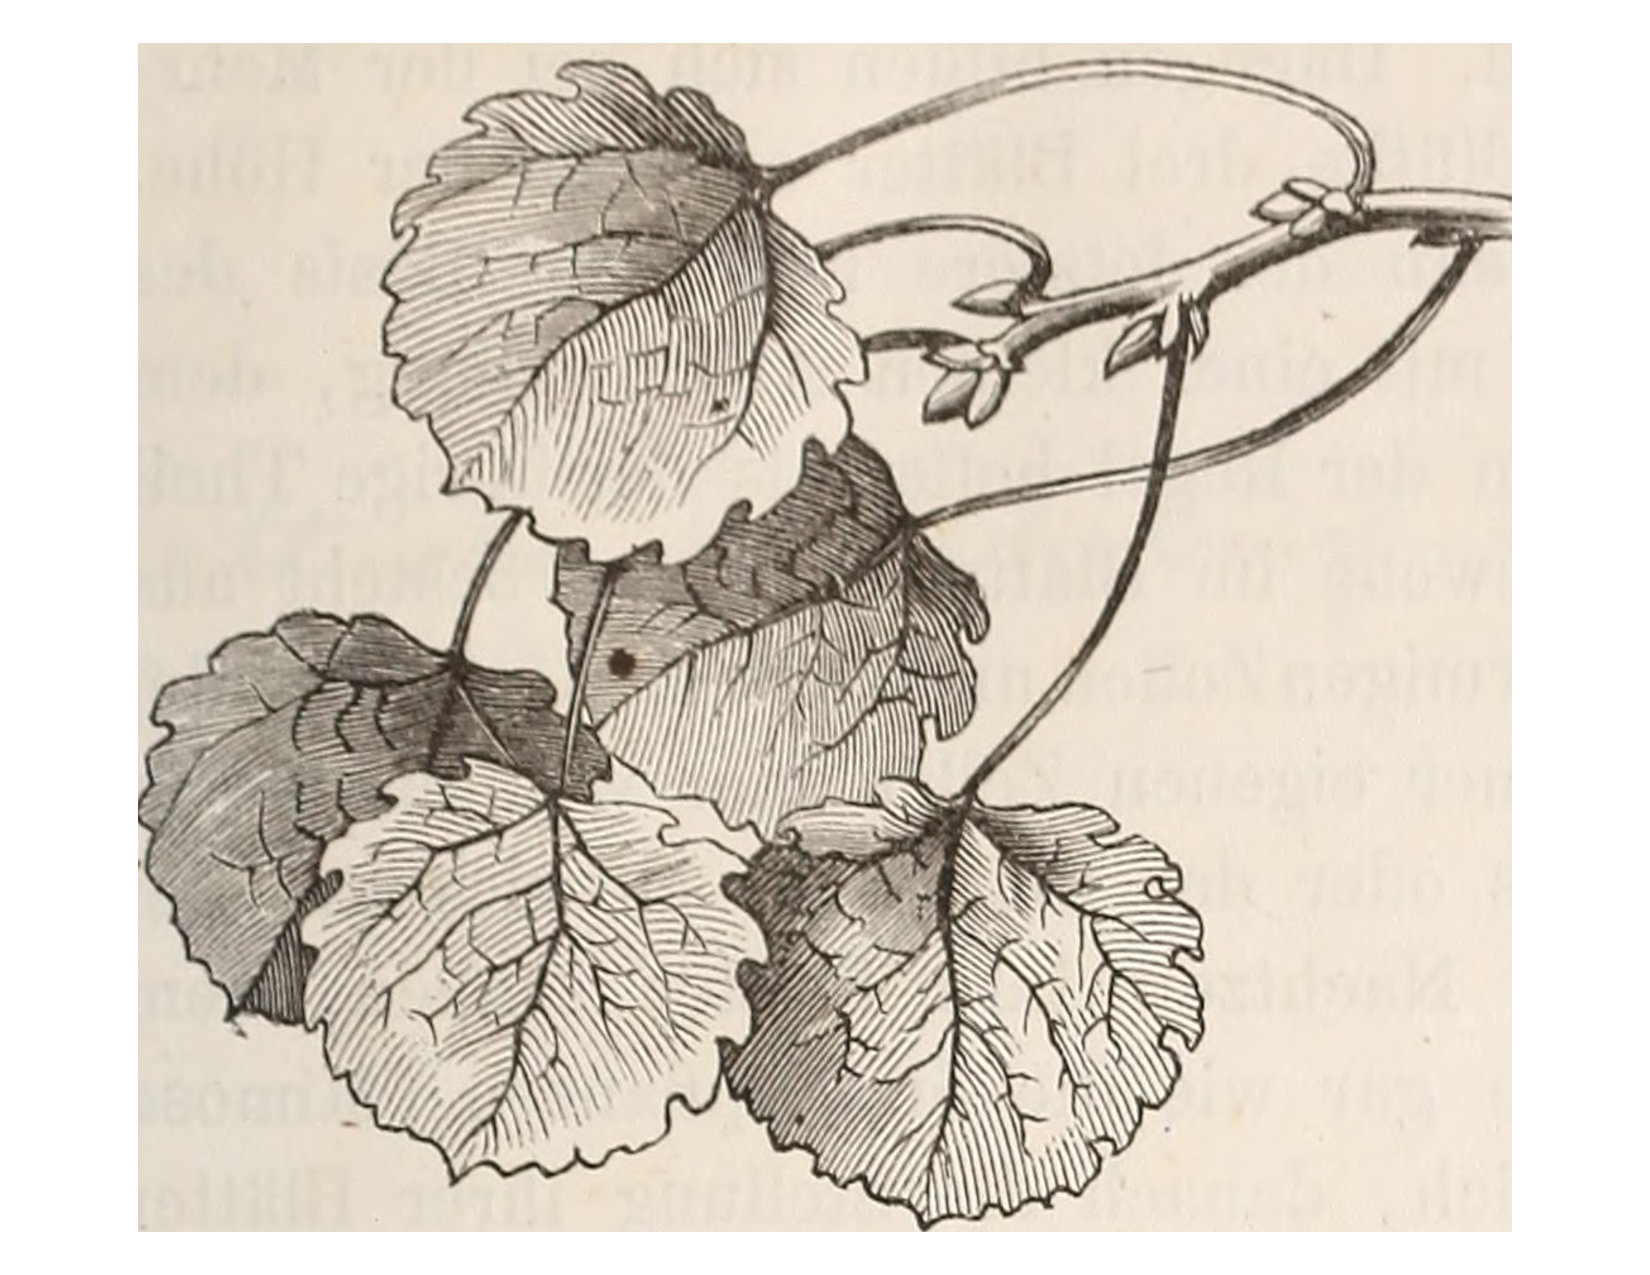
\includegraphics[width=0.8 \textwidth]{illustration_images/Quant_gen/Aspen_budset/Aspen_leaves.pdf}
\end{center}
\caption{European aspen {\it P. tremula}. \BHLNC{Der baum. H. Schacht. 1860. BHL}{https://archive.org/stream/derbaum00scha/\#page/n284/mode/1up}{The Library of Congress} } \label{fig:Apsen}
\end{marginfigure}   Your height, to the amount of
RNA transcribed from a given gene, to what you ate last Tuesday: all
of these are phenotypes.  Nearly any phenotype we can choose to measure about an organism represents the outcome of the information encoded by their genome played out through an incredibly complicated
developmental, physiological and/or behavioural processes that in turn interact with a myriad of environmental and
stochastic factors. Honestly it boggles the mind how organisms work as well as they do, let alone that I managed to eat lunch last Tuesday. 

\begin{marginfigure}[-1cm]
\begin{center}
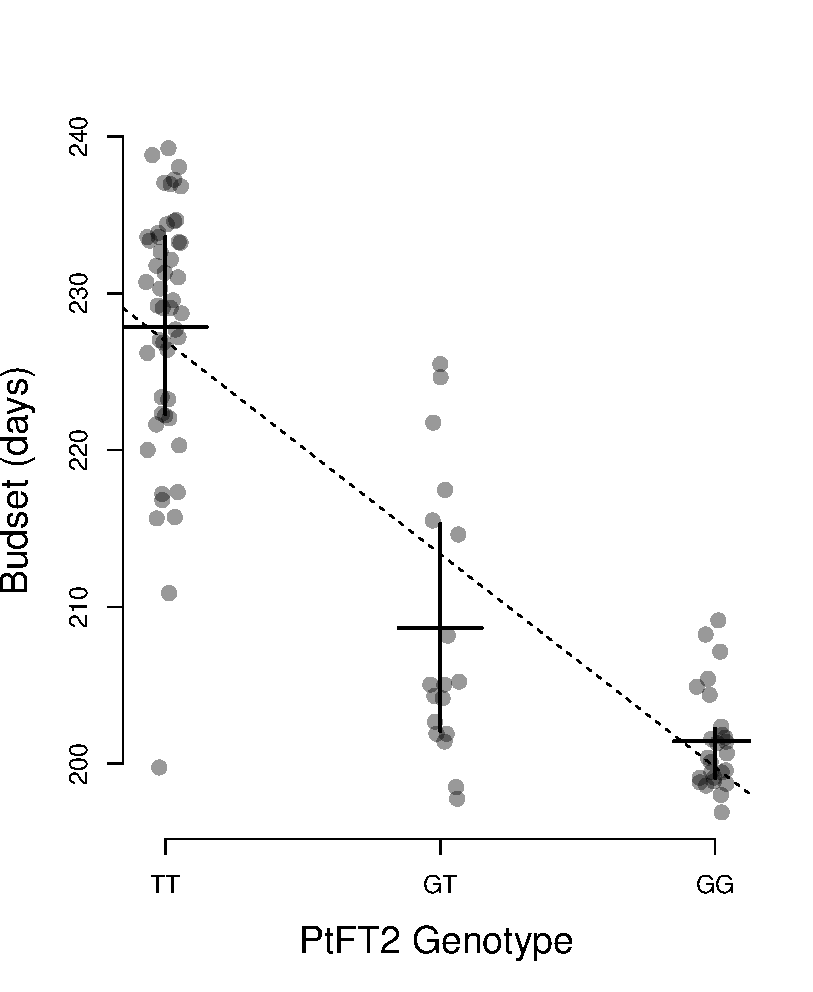
\includegraphics[width=\textwidth]{Journal_figs/Quant_gen/Wang_GWAS_poplar/Poplar_Aspen_budset_geno_pheno.pdf}
\end{center}
\caption{The effect of a flowering time gene (PtFT2) SNP on budset time in European aspen. Each dot gives the genotype-phenotype combination for
  an individual. The horizontal lines give the budset mean for each
  genotype and the vertical lines show the inter-quartile range. The
  dotted line gives the linear regression of phenotype on genotype.
  Thanks to P{\"a}r Ingvarsson for sharing these data from  \citet{wang:18}. } \label{fig:Apsen_geno_pheno}
\end{marginfigure}

There are many different ways to think about studying the path from genotype through to phenotype. The one we will take here is to think about how phenotypic variation among individuals in a population arises as a result of genetic variation in the population.  One simple way to measure this genotype-phenotype relationship is to calculate the phenotypic mean for each genotype at a locus. For example, \citet{wang:18} explored the genetic basis of budset time in European aspen  ({\it Populus tremula}); the effect
of one specific SNP on that phenotype is shown in
in Figure \ref{fig:Apsen_geno_pheno}. Budset timing is a key trait underlying local adaptation to varying growing season length. The associated SNP
falls in a gene (PtFT2) that is known to play a strong role in flowering
time regulation in other plants. 



One way for us to assess the relationship between
genotype and phenotype is to find the best fitting linear line through the data, i.e. fit a linear regression of
phenotypes for our individuals on their genotypes at a particular SNP ($l$):
\begin{equation}
X \sim \mu + a_l G_{l}
\end{equation}
\marginnote{We'll encounter linear regressions at various points
  during the next few chapters, see the math appendix
around eqn \ref{eqn:def_linear_regression} for more background
details.} 
In the equation above, $X$ is a vector of the phenotypes of a set of individuals and $G_{l}$ is our vector of genotypes at locus $l$, with $G_{i,l}$ taking the value 0, 1, or 2 depending on whether our individual $i$ is homozygote, heterozygote, or the alternate homozygote at our locus of interest. Here $\mu$ is our phenotypic mean. The slope of this regression line ($a_l$) has the interpretation of being the average
effect of substituting a copy of allele $2$ for a copy of allele
$1$. In our Aspen example the slope is $-13.6$, i.e. swapping a single $T$ for a $G$ allele
moves the budset forward by $13.6$ days, such that the $GG$ homozygote
is predicted to set buds $27.2$ days earlier than the $TT$ homozygote.   


As a measure of the significance of this genotype-phenotype relationship, we can
calculate the p-value of our regression. To try and identify loci
that are associated with our trait genome-wide, we can conduct this
regression at each SNP we genotype in the genome. One common way to display the
results of such an analysis (called a genome-wide association study or GWAS for short) is to plot the logarithm of the p-value for each SNP along
genome (a so-called Manhattan plot). Here's one from 
\citet{wang:18} for their Aspen budset phenotype


\begin{figure}
\begin{center}
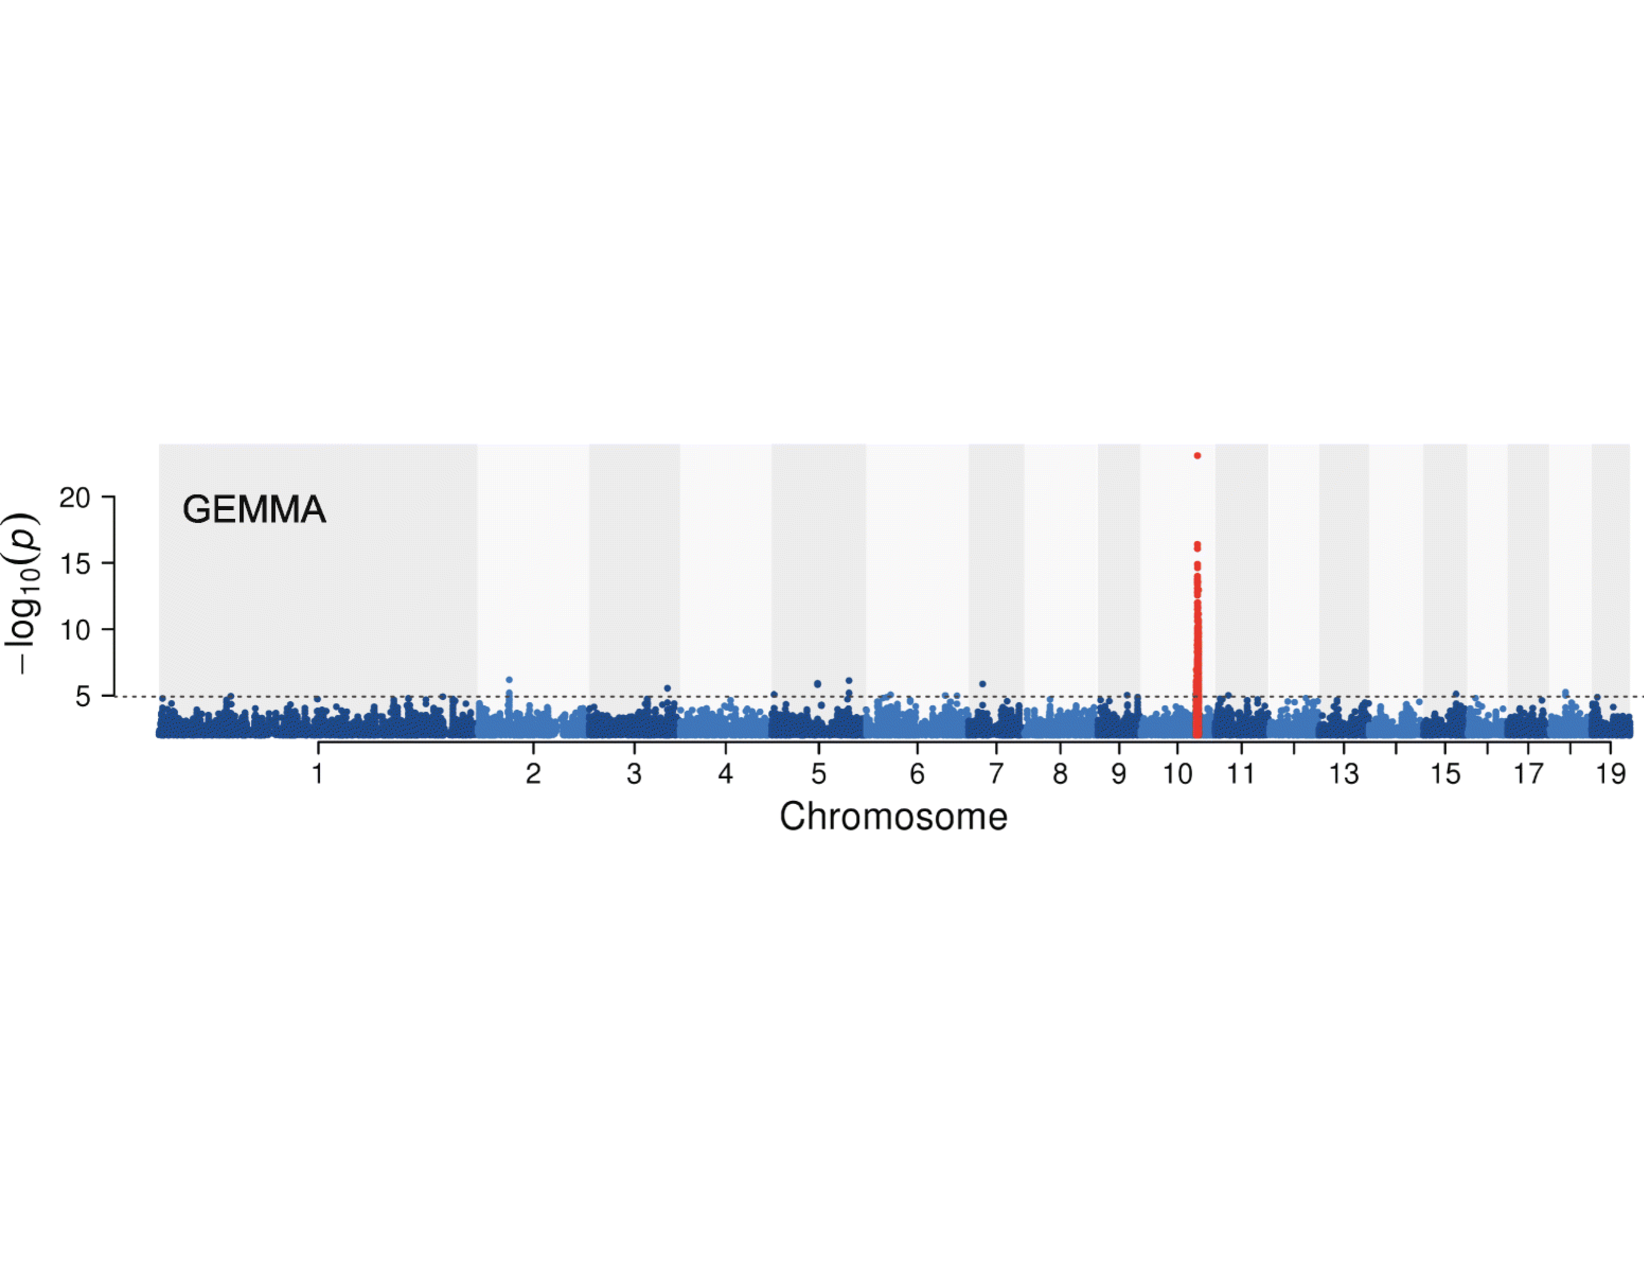
\includegraphics[width=\textwidth]{Journal_figs/Quant_gen/Wang_GWAS_poplar/Wang_Fig_just_Manhattan.pdf}
\end{center}

\caption{Manhattan plot of the p-value of the linear association
  between genotype and budset in Aspen. Each dot represents the test at a single SNP,
  plotted at its physical coordinate in the genome. Different chromosomes
  are plotted in alternating colours. The SNPs surrounding the PtFT2
  gene are shown in red. From \citet{wang:18}, \PLOSccBY. } \label{fig:Apsen_Manhattan}
\end{figure}
The SNP with the most significant p-value is the PtFT2 SNP. Note
that other SNPs in the surrounding region also light up as showing a
significant association with budset timing. This is because loci that are in LD with a functional locus may in turn show an
association, not because they directly affect the phenotype, but simply
because the genotypes at the two loci are themselves non-randomly
associated. Below is a zoomed in version (Figure 2 in \citet{wang:18}) with SNPs coloured by the
strength of their LD with the putatively functional SNP.
\begin{figure}
\begin{center}
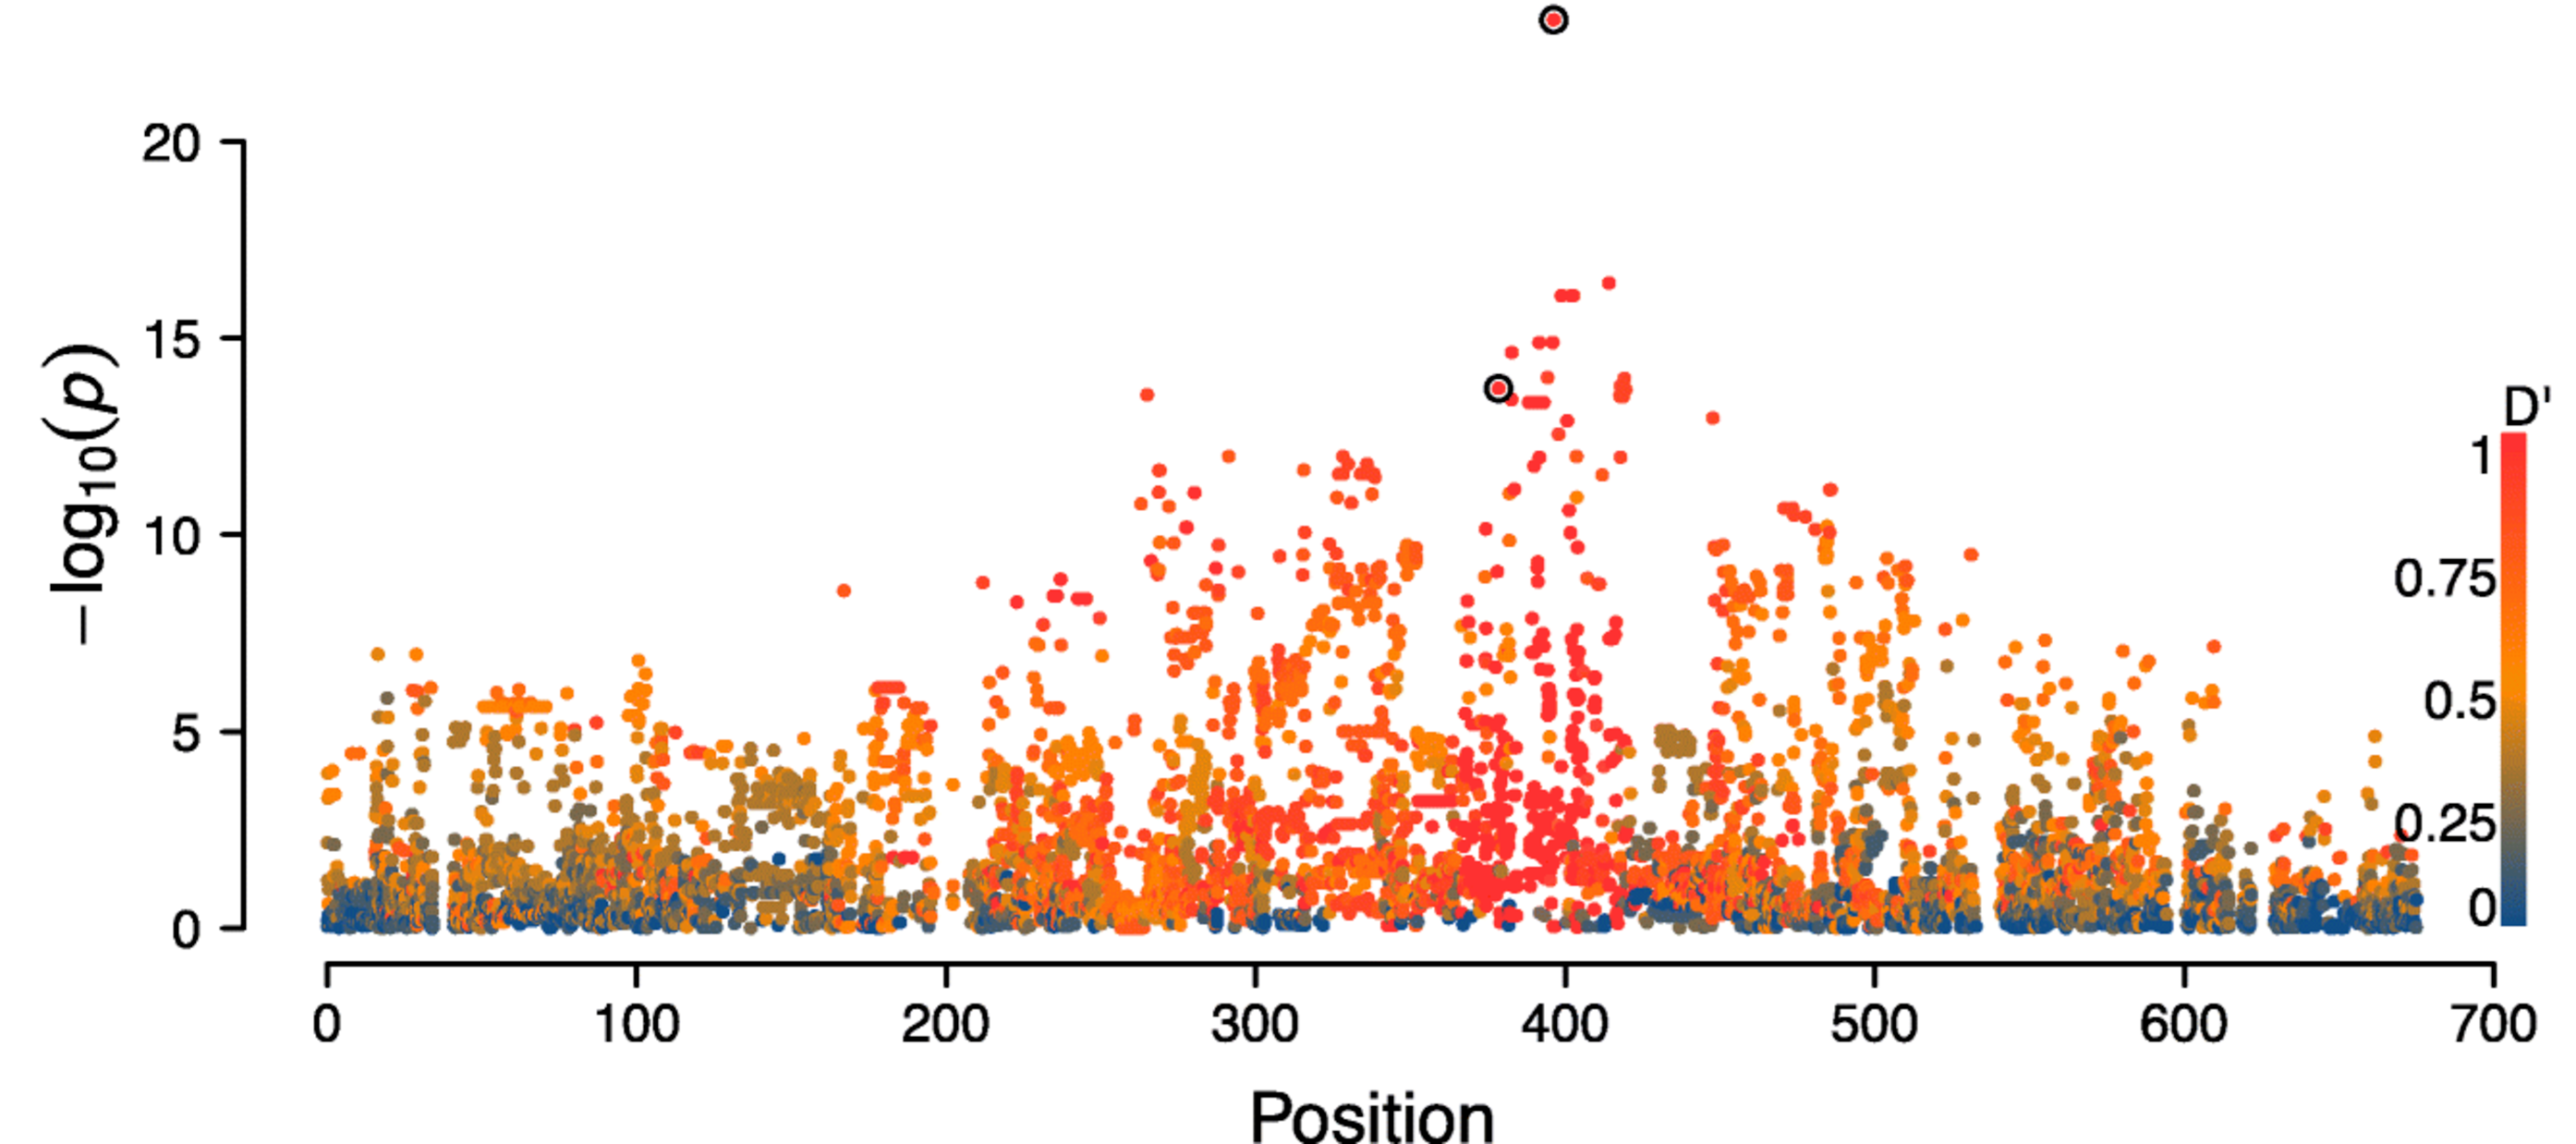
\includegraphics[width=\textwidth]{Journal_figs/Quant_gen/Wang_GWAS_poplar/Wang_Fig_zoomed_Manhattan.pdf}
\end{center}
\caption{The Manhattan plot zoomed in on the top-hit (red SNPs from Figure
  \ref{fig:Apsen_Manhattan}). SNPs are now coloured by their $D\prime$
  value with the most significant SNP. $D\prime$ is the LD
  covariance between a pair of loci ($D$, eqn \eqref{eqn:LD_def}) normalized by
  the largest value $D$ can take given the allele frequencies. Figure from \citet{wang:18},  \PLOSccBY. } \label{fig:Apsen_zoom_Manhattan}
\end{figure}
Note how SNPs in strong LD with the functional allele (redder
points) have more significant p-values. 

Variation in some traits seems to have a relatively simple genetic
basis. In our Aspen example there is one clear large-effect locus,
which explains  62\% of the variation in budset. Note that even in this case, where we have an allele with a very strong effect on a phenotype, this is not an allele {\it for} budset, nor is PtFT2 a gene {\it for} budset. \marginnote{
``All that we mean when we speak of a gene [allele] for pink eyes is, a gene which differentiates a pink eyed fly 
from a normal one \textemdash not a gene [allele] which produces pink eyes per se, for the character pink eyes is dependent 
on  the action of many other genes." - \citet{sturtevant:15}
} It is an allele that is associated with budset in the sampled environments and populations. In a different set of environments, this allele's effects may be far smaller, and a different set of alleles may contribute to phenotype variation. PtFT2, the gene our focal SNP falls close to, is just one of many genes and molecular pathways involved in budset. A mutant screen for budset may uncover many genes with larger effects; this gene is just a locus that happens to be polymorphic in this particular set of genotyped individuals. 

While phenotypic variation for some phenotypes has a relatively simple genetic basis, many phenotypes are likely much more genetically complex, involving the functional effect of many alleles at hundreds or thousands of polymorphic loci. For example hundreds of small effect loci affecting human height have been mapped in European populations to date. Such genetically complex traits are called polygenic traits. 

In this chapter, we will use our understanding of the sharing of alleles between relatives to understand the phenotypic resemblance between relatives in
quantitative phenotypes. This will allow us to understand the contribution of genetic variation to phenotypic variation. In the next chapter, we will then use these results to understand the evolutionary change in quantitative phenotypes in response to selection. \\

\subsection{A simple additive model of a trait}
Let's imagine that the genetic component of the variation in our trait is controlled by $L$ autosomal loci that act in an additive manner. The frequency of allele $1$ at locus $l$ is $p_l$, with each copy of allele $1$ at this locus increasing your trait value by $a_l$ above the population mean.
The phenotype of an individual, let's call her $i$, is $X_i$.
Her genotype at SNP $l$ is
$G_{i,l}$. Here $G_{i,l}=0,~1,$ or $2$,  representing the number of copies of allele $1$ she
has at this SNP. Her expected phenotype, given her genotype at all $L$ SNPs, is then
\begin{equation}
\E (X_i | G_{i,1},\cdots,G_{i,L}) =\mu + X_{A,i} = \mu+\sum_{l=1}^L G_{i,l} a_{l} \label{pheno_geno}
\end{equation}
where $\mu$ is the mean phenotype in our population, and $X_{A,i}$ is
the deviation away from the mean phenotype due to her genotype. Now in reality the phenotype is a function of the
expression of those alleles in a particular environment. Therefore, we
can think of this expected phenotype as being an average across a set
of environments that occur in the population. \\

%\gc{NEED to resolve $\mu$ in above equation}


When we measure our individual's observed phenotype we see
\begin{equation}
X_i =   \mu+X_{A,i} + X_{E,i} \label{pheno_geno_environ}
\end{equation}
where $X_E$ is the deviation from the mean phenotype due to the
environment. This $X_E$ includes the systematic effects of the environment
our individual finds herself in and all of the noise during
development, growth, and the various random insults that life throws
at our individual. If a reasonable number of loci contribute to
variation in our trait then we can approximate the distribution of
$X_{A,i}$ by a normal distribution due to the central limit theorem
(see Figure \ref{fig:QT1}). \sidenote{The central limit theory is
  discussed briefly in the math appendix section \ref{section:useful_limits}.} Thus if we can
approximate the distribution of the effect of environmental variation
on our trait ($X_{E,i}$) also by a normal distribution, which is
reasonable as there are many small environmental effects, then the
distribution of phenotypes within the population ($X_i$) will be
normally distributed (see Figure \ref{fig:QT1}).\\

\begin{figure}
\begin{center}
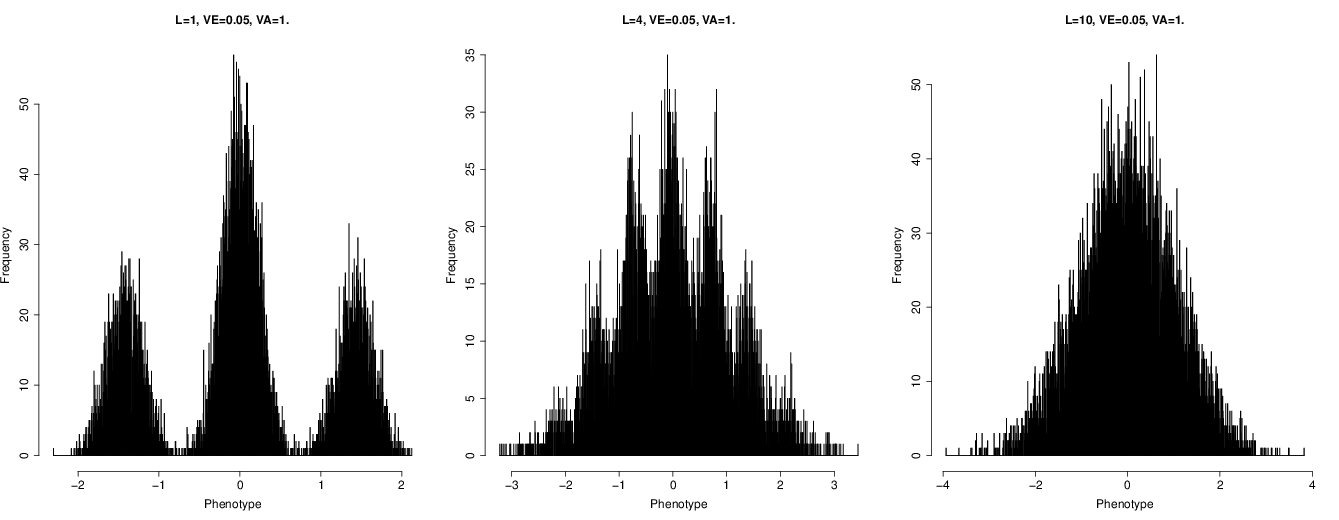
\includegraphics[width=\textwidth]{figures/QT1.png}
\end{center}
\caption{The convergence of the phenotypic distribution to a normal
  distribution. Each of the three histograms shows the distribution of
the phenotype in a large sample, for increasingly large numbers of loci ($L=1,~4,$ and $10$, with the proportion of variance explained held at $V_A=1$). I have simulated each individual's
phenotype following equations \ref{pheno_geno} and \ref{pheno_geno_environ}. Specifically, we've simulated each
individual's biallelic genotype at $L$ loci, assuming Hardy-Weinberg proportions
and that the allele is at 50\% frequency. We assume that all of the
alleles have equal effects and combine them additively together. We then add an environmental contribution, which is normally distributed with variance $0.05$. Note that in the left two pictures you can see peaks
corresponding to different genotypes due to our low  environmental
noise (in practice we can rarely see such peaks for real quantitative phenotypes). \gitcode{https://github.com/cooplab/popgen-notes/blob/master/Rcode/Quant_gen/QT1.R}} \label{fig:QT1}
\end{figure}
\graham{Add IGF1 dog eg?}
Note that as this is an additive model; we can decompose eqn. \ref{pheno_geno_environ} into the
effects of the two alleles at each locus and rewrite
it as
\begin{equation}
X_i = \mu + X_{iM}+X_{iP} +X_{iE}
\end{equation}
where $X_{iM}$ and $X_{iP}$ are the contribution to the phenotype of
the alleles that our individual received from her mother (maternal
alleles) and father (paternal alleles) respectively. This will come in
handy in just a moment when we start thinking about the phenotypic covariance of relatives.\\

Now obviously this model seems silly at first sight as alleles don't only act in an additive manner, as they interact with alleles at the same loci (dominance) and at different loci (epistasis). Later we'll relax this assumption, 
however, we'll find that if we are interested in evolutionary change over short time-scales it is actually only the ``additive
component'' of genetic variation that will (usually) concern us. 
We will define this more formally later on, but for the moment 
we can offer the intuition that parents only get to pass on a single allele at each locus on to the next generation. As such, it is the effect of these transmitted alleles, averaged over possible matings, that is an individual's average contribution  to the next generation (i.e. the additive effect of the alleles that their genotype consists of).



\subsection{Additive genetic variance and heritability}
As we are talking about an additive genetic model, we'll talk about the additive genetic variance ($V_A$), the phenotypic variance due to the additive effects of segregating genetic variation. This is a subset of the total genetic
variance if we allow for non-additive effects. \\

The variance of our phenotype across individuals ($V$) we can write as
\begin{equation}
V = Var(X_A) + Var(X_E) = V_A+V_E
\end{equation}
In writing the phenotypic variance as a sum of the additive and
environmental contributions, we are assuming that there is no
covariance between $X_{G,i}$ and $X_{E,i}$ i.e. there is no covariance
between genotype and environment. \sidenote{In this section we're making use of
  the properties of the variance of a random variable, see math
  appendix eqn \eqref{eqn:general_var_decomp}} \\

Our additive genetic variance can be written as
\begin{equation}
V_A = \sum_{l=1}^L Var(G_{i,l} a_{l})
\end{equation}
where $Var(G_{i,l} a_{l})$ is the contribution of locus $l$ to the additive
variance among individuals. Assuming random mating, and that our loci are in linkage equilibrium, we can write our additive genetic variance as
\begin{equation}
V_A = \sum_{l=1}^L a_{l}^2 2 p_l(1-p_l)  \label{eqn:VA}
\end{equation}
where the $ 2 p_l(1-p_l)$ term follows from the binomial sampling of
two alleles per individual at each locus. \sidenote{These results follow from
  the properties of variance in math appendix eqn \eqref{eqn:general_var_decomp}. }\\

\begin{question}
You have two biallelic SNPs contributing to variance in human height. At the first SNP you have an allele with an additive effect of $5$cm which is found at a frequency of $\nicefrac{1}{10,000}$. At the second SNP you have an allele with an additive effect of $-0.5$cm segregating at 50\% frequency. Which SNP contributes more to the additive genetic variance? Explain the intuition of your answer.
\end{question}
\paragraph{An example of the additive basis of variation using polygenic scores.}
Now we don't usually get to see the individual loci contributing to
highly polygenic traits. Instead, we only get to see the distribution
of the trait in the population. However, with the advent of GWAS in
human genetics we can see some of the underlying genetics using the
many trait-associated loci identified to date. Using the estimated
effect sizes at each locus, each one of which is tiny, we can
calculate the weighted sum over an individual's genotype as in
equation \ref{pheno_geno}. This weighted sum is called the
individual's polygenic score. To illustrate how polygenic scores work,
we can take a set of 1700 SNPs\sidenote{each chosen as the SNP with the strongest signal of association with height in 1700 roughly independent bins spaced across the genome}. The effects of these SNPs are tiny; the median, absolute additive effect size is $0.07$cm. Figure \ref{fig:Biobank_height_PGS} shows the distribution of a thousand individuals' polygenic scores calculated using these 1700 SNPs (simulated genotypes using the UKBB frequencies). The standard deviation of these polygenic scores $\sim 2$cm. 
The individuals with higher polygenic scores for height are predicted to be taller than the individuals with lower polygenic scores. 
\begin{figure}
\begin{center}
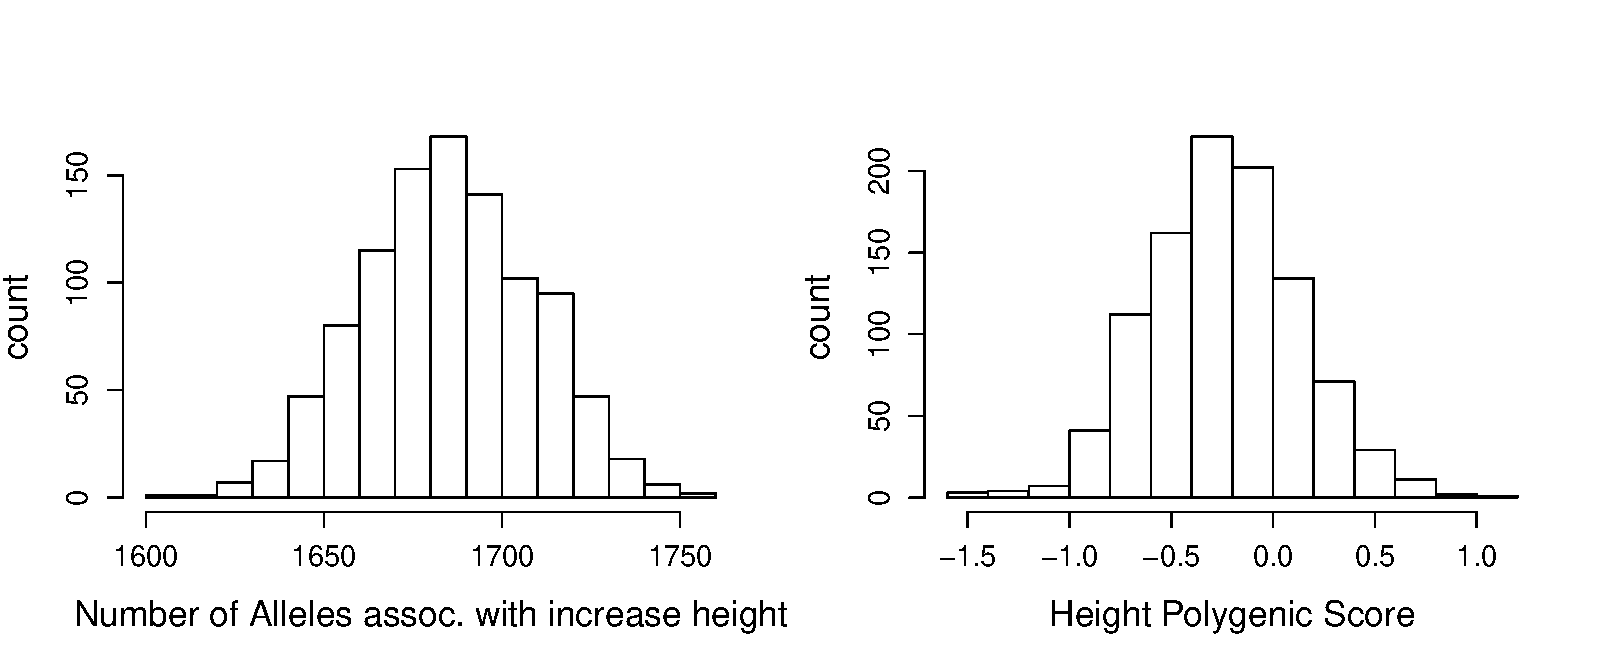
\includegraphics[width=\textwidth]{figures/Biobank_height_dist.pdf}
\end{center}
\caption{{\bf Left)} The distribution of the number of
  height-increasing alleles that individuals carry at 1700 SNPs
  associated with height in the UK Biobank, for a sample of 1000
  individuals. {\bf right)} The distribution of the polygenic scores
  for these 1000 individuals. Plotted on top is a normal distribution
  with the same mean and variance. The empirical variance of these
  polygenic scores is $0.13$, the additive genetic variance calculated
  by equation \eqref{eqn:VA} is $0.135$, so the two are in good
  agreement. \gitcode{https://github.com/cooplab/popgen-notes/blob/master/Rcode/Height/Biobank_height.R} } \label{fig:Biobank_height_PGS}
\end{figure}
 

\paragraph{The narrow sense heritability}
We would like a way to think about what proportion of the variation
in our phenotype across individuals is due to genetic differences as
opposed to environmental differences. Such a quantity will be key in
helping us think about the evolution of phenotypes. For example, if
variation in our phenotype had no genetic basis, then no matter how
much selection changes the mean phenotype within a generation
the trait will not change over generations. \\

We'll call the proportion of the variance that is genetic the
\textit{heritability}, and denote it by $h^2$. We can then write heritability as
\begin{equation}
h^2 = \frac{Var(X_A)}{V} = \frac{V_A}{V}
\end{equation}
Remember that we are thinking about a trait where all of the alleles act
in a perfectly additive manner. In this case our heritability $h^2$ is
referred to as the \textit{narrow sense heritability}, the proportion of the
variance explained by the additive effect of our loci.
When we allow dominance
and epistasis into our model, we'll also have to define the \textit{broad sense
heritability} (the total proportion of the phenotypic variance
attributable to genetic variation).\\

The narrow sense heritability of a trait is a useful quantity; indeed
we'll see shortly that it is exactly what we need to understand the
evolutionary response to selection on a quantitative phenotype. We can
calculate the narrow sense heritability by using the resemblance between
relatives. For example, if the phenotypic differences between individuals in our population were solely determined by environmental differences experienced by these different individuals, we
should not expect relatives to resemble each other any more than random
individuals drawn from the population. Now the obvious caveat here is
that relatives also share an environment, so may resemble each other
due to shared environmental effects. \\

Note that the heritability is a property of a sample from the population in a particular set of environments at a particular time. Changes in the environment may change the phenotypic variance. Changes in the environment may also change how our genetic alleles are expressed through development and so change $V_A$. Thus estimates of heritability are not transferable across environments or populations. 



 
\subsection{The covariance between relatives}
People have long been fascinated by the resemblance between relatives,
particularly twins (see Figure
\ref{Fig:The_Cholmondeley_Ladies}). Families hold a special place in
quantitative genetics, as remarkably we can use the
resemblance between relatives to directly estimate the heritability
and covariance of traits. To see this we can calculate the covariance in phenotype between two individuals
($1$ and $2$) who have phenotypes $X_1$ and $X_2$
respectively.\sidenote{We'll be dealing with covariance a lot this
  chapter, see math appendix section \ref{section:multi_RV} for more background.} To
think about imagine plotting the phenotypes of, say, sisters against
each other. The x and y coordinates of each point will be the, say,
heights of the pair of siblings. Do tall women tend to have tall
sisters, do short women tend to have short sisters? How much do their
phenotypes covary. If some of the variation in our phenotype is
genetic we expect identical twins to resemble each other more than
full siblings, who in turn will resemble each other more than
half-sibs and so on out (see Figure \ref{fig:Varying_rellys_phenos}). Under our simple additive model of phenotypes we
can write the covariance as 
\begin{equation}
Cov(X_1,X_2) =
Cov\left((X_{1M}+X_{1P}+X_{1E}),((X_{2M}+X_{2P}+X_{2E}) \right)
\end{equation}
We can expand this out in terms of the covariance between the various
components in these sums.\\

\begin{figure}
 \begin{center}
 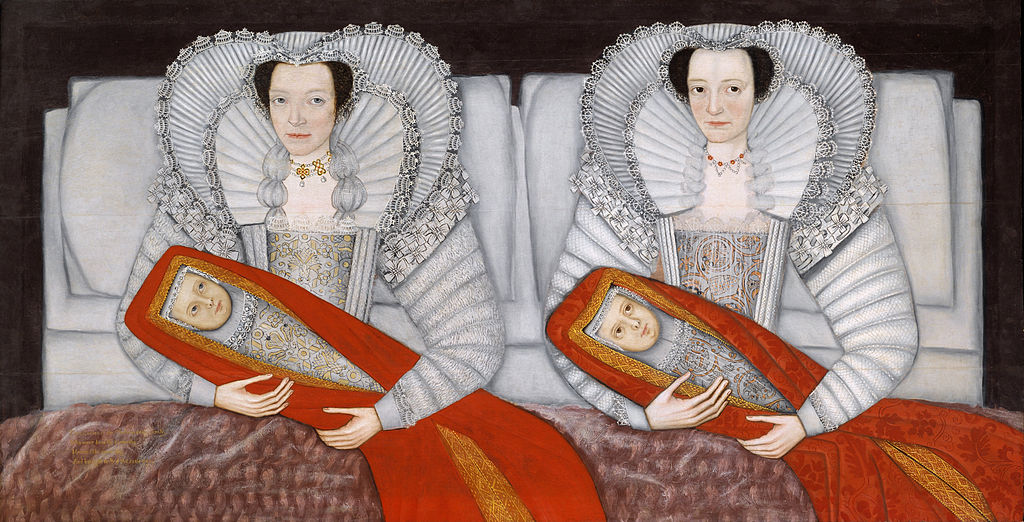
\includegraphics[width=\textwidth]{illustration_images/Quant_gen/Cholmondeley_Ladies/1024px-British_School_17th_century_-_The_Cholmondeley_Ladies_-_Google_Art_Project.jpg}
 \end{center}

  \caption{The Cholmondeley Ladies. Unknown British Painter, circa
    1600. Inscription on bottom left of the painting ``Two Ladies of
    the Cholmondeley Family, Who were born the same day, Married the
    same day, And brought to Bed the same day.'' The ladies are
    thought to be twin sisters, but there's a clue that they're not
    identical twins. Can you spot it?
    \newline \noindent  \tiny{  Image from
      \href{https://commons.wikimedia.org/wiki/File:British_School_17th_century_-_The_Cholmondeley_Ladies_-_Google_Art_Project.jpg}{Wikimedia},
      considered public domain in the United States, UK
      \href{https://www.tate.org.uk/art/artworks/unknown-artist-britain-the-cholmondeley-ladies-t00069}{Tate}
      \textcopyright Creative Commons
      CC-BY-NC-ND (3.0 Unported)}} \label{Fig:The_Cholmondeley_Ladies}
   \end{figure}

To make our task easier, we will make two commonly made assumptions:
\begin{enumerate}
\item We can ignore the covariance of the environments
between individuals (i.e. $Cov(X_{1E},X_{2E})=0$)
\item We can ignore the covariance
between the environment of one individual and the
genetic variation in another individual (i.e. $Cov(X_{1E},(X_{2M}+X_{2P}))=0$). (We can actually incorporate these effects in later if we choose too.)
\end{enumerate}

The failure of these assumptions
to hold can undermine our estimates of heritability, but we'll
return to that later. Moving forward with these assumptions, we can
simplify our original expression above and write our phenotypic covariance between our pair of individuals as
\begin{equation}
Cov(X_1,X_2) =
Cov((X_{1M},X_{2M})+Cov(X_{1M},X_{2P})+Cov(X_{1P},X_{2M})
+Cov(X_{1P},X_{2P}) \label{cov_rels_1}
\end{equation}
This equation is saying that, under our simple additive model, we can see the
covariance in phenotypes between individuals as the covariance between
the maternal and paternal allelic effects in our individuals. We can use our results about
the sharing of alleles between relatives to obtain these covariance terms.
But before we write down the general case, let's quickly work through some
examples. \\

 \begin{figure*}
 \begin{center}
 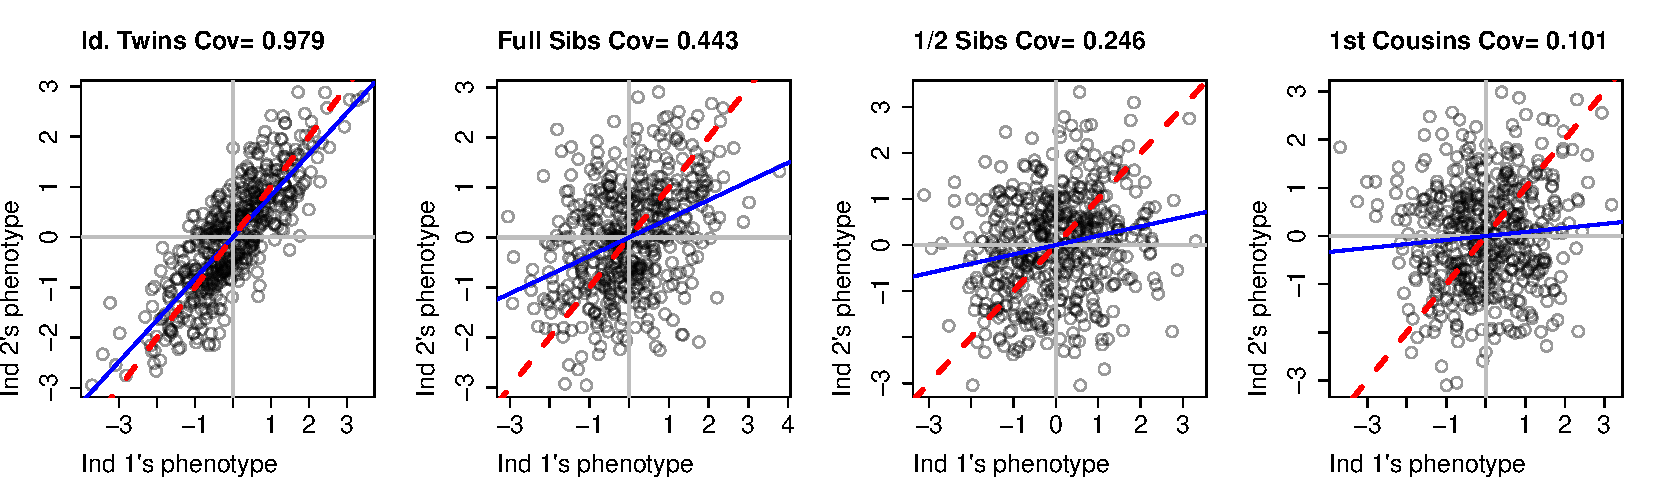
\includegraphics[width=\textwidth]{figures/Varying_rellys_phenos.pdf}
 \end{center}
 \caption{Covariance of phenotypes between pairs of individuals of a
   given relatedness. Each point gives the phenotypes of a different
   pair of individuals. The additive genetic variance is held constant
   at $V_A=1$, such that the expected covariances ($2F_{1,2}V_A$)
   should be $1$, $0.5$, $0.25$, and $0.125$ respectively in good agreement with
   the empirical covariances reported in the title of each graph. The
   data were simulated as described in
 the caption of Figure \ref{fig:QT1}. The dashed red line shows $x=y$ and the solid blue
line shows the best fitting linear regression line. \gitcode{https://github.com/cooplab/popgen-notes/blob/master/Rcode/Quant_gen/QT4.R}}\label{fig:Varying_rellys_phenos}
 \end{figure*}
 
\paragraph{The covariance between identical twins}
Let's first consider the case of a pair of identical twins, monzygotic
(MZ) twins, from two
unrelated parents. Our pair of twins share their maternal and paternal
allele identical by descent ($X_{1M}=X_{2M}$ and $X_{1P}=X_{2P}$). As their maternal and
paternal alleles are not correlated draws from the population,
i.e. have no probability of being $IBD$ as we've said the parents are unrelated, the
covariance between their effects on the phenotype is zero  
(i.e. $Cov(X_{1P},X_{2M})=Cov(X_{1M},X_{2P})=0$). In that case,
eqn. \ref{cov_rels_1} is
\begin{equation}
Cov(X_1,X_2) = Cov((X_{1M},X_{2M})+Cov(X_{1P},X_{2P}) = 2Var(X_{1M})
= V_A
\end{equation}
To calculate the narrow sense heritability we could then in principal divide the
covariance of our pairs of MZ  twins (MZ$_1$ and MZ$_2$) by the trait variance to give
\begin{equation}
h^2 = \frac{Cov(\text{MZ}_1, \text{MZ}_2) }{V} =
\rho_{\text{MZ}}
\end{equation}
where $\rho_{\text{MZ}}$ is the correlation of pairs of MZ twins (see
Appendix eqn \eqref{eqn:def_corr} for more on correlations).
For example, we could estimate the heritability of a measure of body
from the MZ correlation in Figure \ref{fig:twins_body_fat}. In general, this simple estimator isn't great as the correlation of
identical twins includes the effects of the shared family
environment of the twins (i.e. $Cov(X_{1E},X_{2E})$).
 \begin{marginfigure}
 \begin{center}
 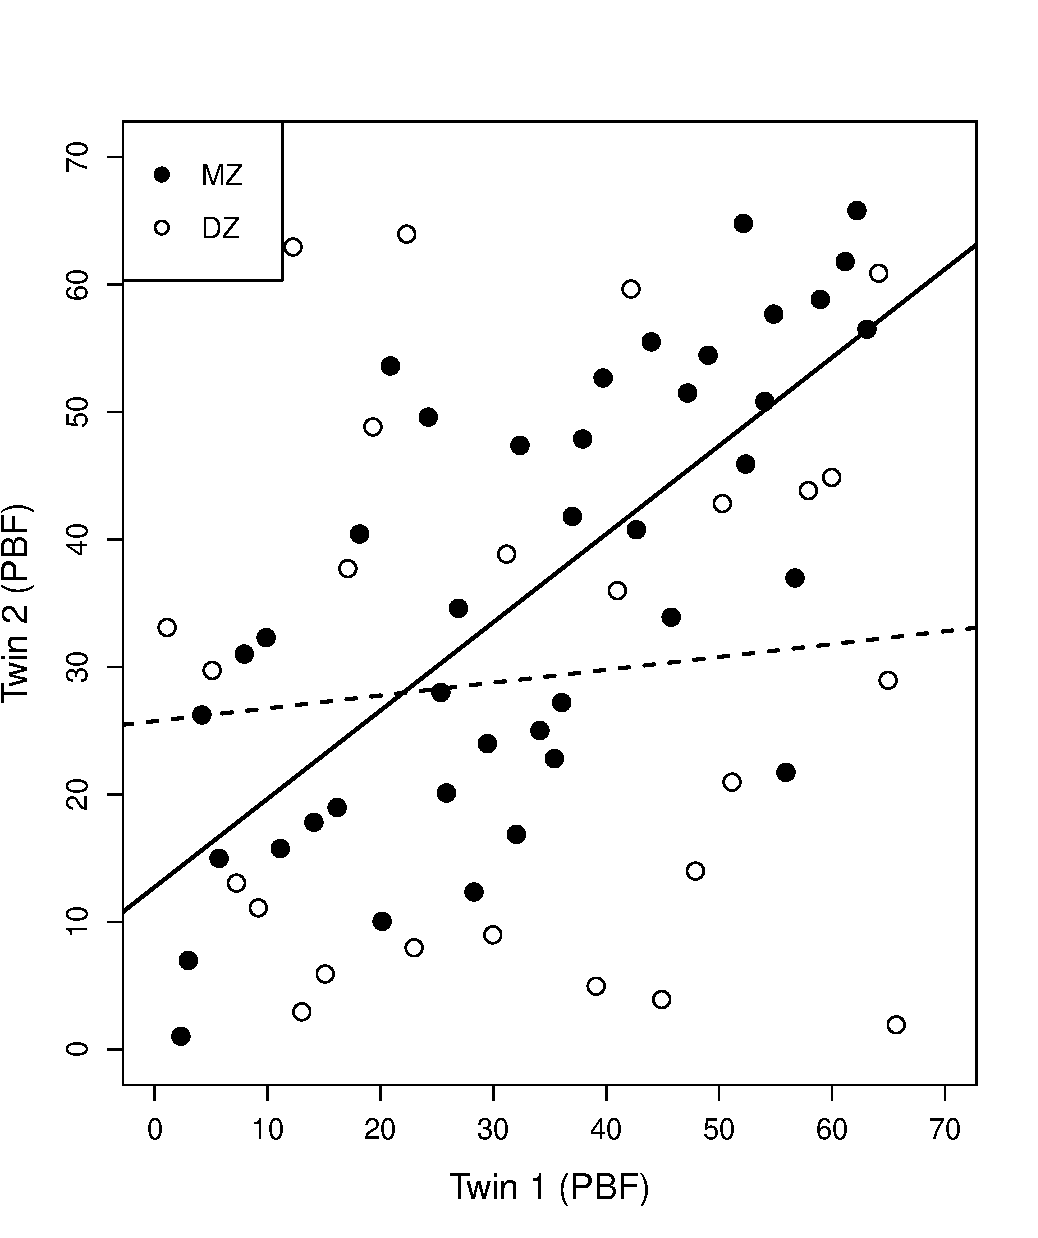
\includegraphics[width=\textwidth]{Journal_figs/Quant_gen/twins_body_fat/twins_body_fat.pdf}
 \end{center}
 \caption{A measure of body fat in pairs of Monozygotic (MZ) and
   Dizygotic (DZ) twins. Our sample  correlations are
   $\hat{\rho}_{\text{MZ}}=0.72$ and $\hat{\rho}_{\text{MZ}}=0.10$. Data from \citet{faith1999evidence}, \gitcode{https://github.com/cooplab/popgen-notes/blob/master/Journal_figs/Quant_gen/twins_body_fat/twins_body_fat.R}}\label{fig:twins_body_fat}
 \end{marginfigure}
Moreover, it can
be inflated by non-additive effects as identical twins don't just share alleles, they share their entire genotypes, and thus 
resemble each other in phenotype also because of shared dominance
effects (we'll discuss non-additive effects in Section \ref{section:nonAddVar}). Better twin-based estimates of heritability are commonly
used based on the comparison of MZ vs twins that bypass some of these issues.\\


%% twin bmis https://sci-hub.tw/https://pediatrics.aappublications.org/content/104/1/61.figures-only?sso=1&sso_redirect_count=1&nfstatus=401&nftoken=00000000-0000-0000-0000-000000000000&nfstatusdescription=ERROR%3a+No+local+token

\paragraph{The covariance in phenotype between parent and child}
\begin{marginfigure}
\begin{center}
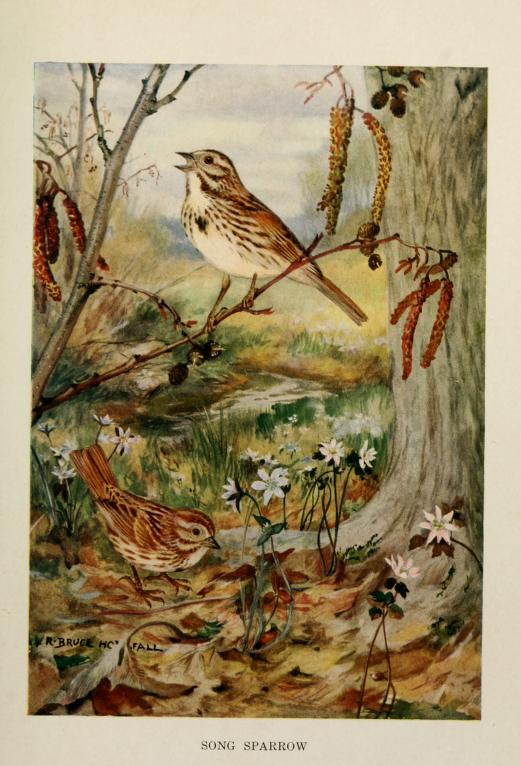
\includegraphics[width=\textwidth]{illustration_images/Quant_gen/song_sparrow/birdbiographies00ball_0165.jpg}
\end{center}
\caption{Song sparrow ({\it Melospiza melodia}). ``He is the most
  incurable optimist of my acquaintance''.
  \BHLNC{Bird biographies (1923). Ball, A.E. illustrations by Horsfall R.B.}{https://www.biodiversitylibrary.org/page/7282967\#page/163/mode/1up}{American Museum of Natural History Library}
} \label{fig:song_sparrow}
\end{marginfigure}
Children resemble their biological parents because children inherit their genome from
their parents (putting aside shared environments for the moment). If a mother and father are unrelated individuals, i.e. are two
random draws from the population, then this mother and her child share
one allele IBD at each locus (i.e. $r_1=1$ and $r_0=r_2=0$). Lets
assume that our mother (ind 1) transmits her paternal allele to the child (ind 2), in which
case $X_{P1}=X_{M2}$, and so $Cov(X_{P1},X_{M2})=Var(X_{P1})=\half
V_A$, and all
the other covariances in eqn. \ref{cov_rels_1} are zero. We'd also
arrive at this result if instead we had thought of the mother transmitting her own
maternal allele. Thus $Cov(X_1,X_2) = \half
V_A$, we can leverage this form of the covariance to directly estimate
$h^2$ by regression.\\
%The other half of the time she transmits her maternal allele to the child, in which case
%$Cov(X_{M1},X_{M2})=Var(X_{M1})$ and all the other terms are zero. 

We can estimate the narrow sense heritability through the regression of child's phenotype on the parental mid-point
phenotype. The parental mid-point phenotype is simply the average of
the mum and dad's phenotype. See Figure \ref{fig:song_sparrow_herit}
for an example from Song sparrows. 

\begin{figure}
\begin{center}
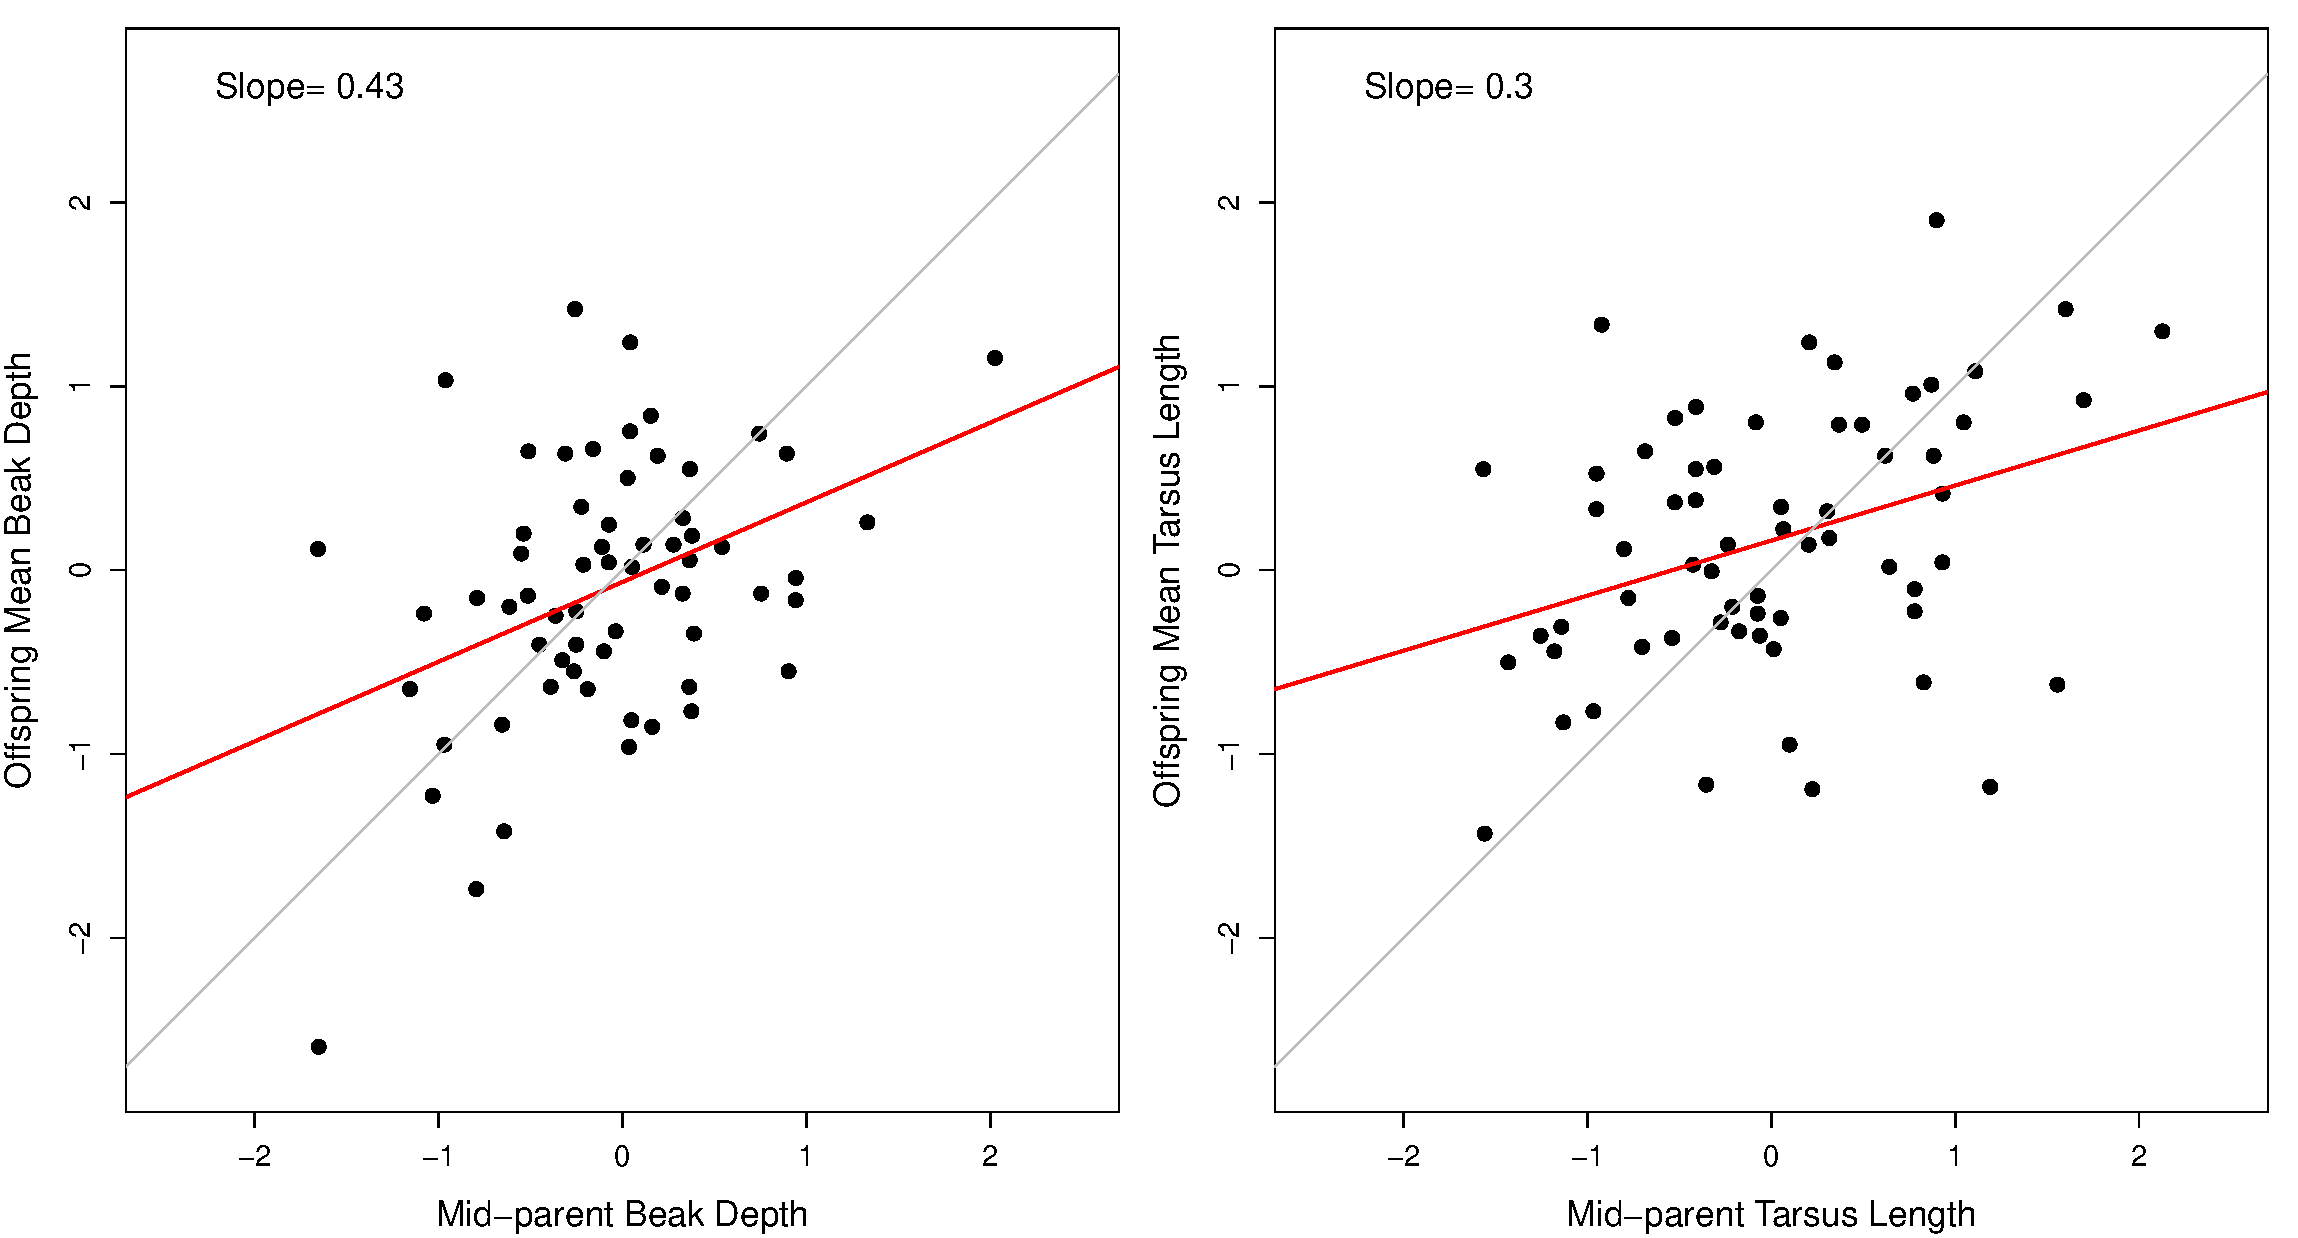
\includegraphics[width=\textwidth]{Journal_figs/Quant_gen/song_sparrow_herit/song_sparrow_herit.pdf}
\end{center}
\caption[][3cm]{Parent-midpoint offspring regression for beak depth and
  tarsus length in song sparrows.  The phenotypes have been standardized to have mean $0$  and variance $1$. The red line shows the best fitting
  slope, whose slope is reported on the graph.  Note that \citet{smith1979heritability}
regressed the average offspring phenotype
for each family on parental mid-point ($X_{\textrm{avg.~kid}}\sim X_{\textrm{mid}}$), as they had multiple offspring per family. However, this doesn't change the slope of the
regression from the form given by eqn \eqref{eqn:par_off_herit}.  The grey line is the
  $x=y$ line. Data from \citet{smith1979heritability},
  \gitcode{https://github.com/cooplab/popgen-notes/blob/master/Journal_figs/Quant_gen/song_sparrow_herit/song_sparrow_herit.R}} \label{fig:song_sparrow_herit}
\end{figure}

We denote the child's phenotype by $X_{kid}$ and mid-point
phenotype by $X_{\textrm{mid}}$, so that if we take the regression $X_{\textrm{kid}} \sim X_{\textrm{mid}}$ this
regression has slope $\beta = Cov(X_{\textrm{kid}},X_{\textrm{mid}})/Var(X_{\textrm{mid}})$.
The covariance of $Cov(X_{\textrm{kid}},X_{\textrm{mid}})=\half
V_A$, and $Var(X_{\textrm{mid}}) = \half V$, as by taking the average of the
parents we have halved the variance, such that the slope of the
regression is
\begin{equation}
\beta_{\textrm{mid}, \textrm{kid}}=
\frac{Cov(X_{\textrm{kid}},X_{\textrm{mid}})}{Var(X_{\textrm{mid}})}=
\frac{V_A}{V} = h^2 \label{eqn:par_off_herit}
\end{equation}
i.e. the regression of the child's phenotype on the parental midpoint
phenotype is an estimate of the narrow sense
heritability.\sidenote{See math appendix eq
  \eqref{eqn:slope_linear_reg} for more on regression slopes.} If much
of the phenotypic variation is due to the (additive) differences in
genotypes among individuals ($h^2 \approx 1$), then children will closely resemble their
parents. Conversely if much of the variation is environmental  ($h^2 \approx 0$), and
there is no shared environment between parent and child, children will
not resemble their parents.

\begin{figure}
\begin{center}
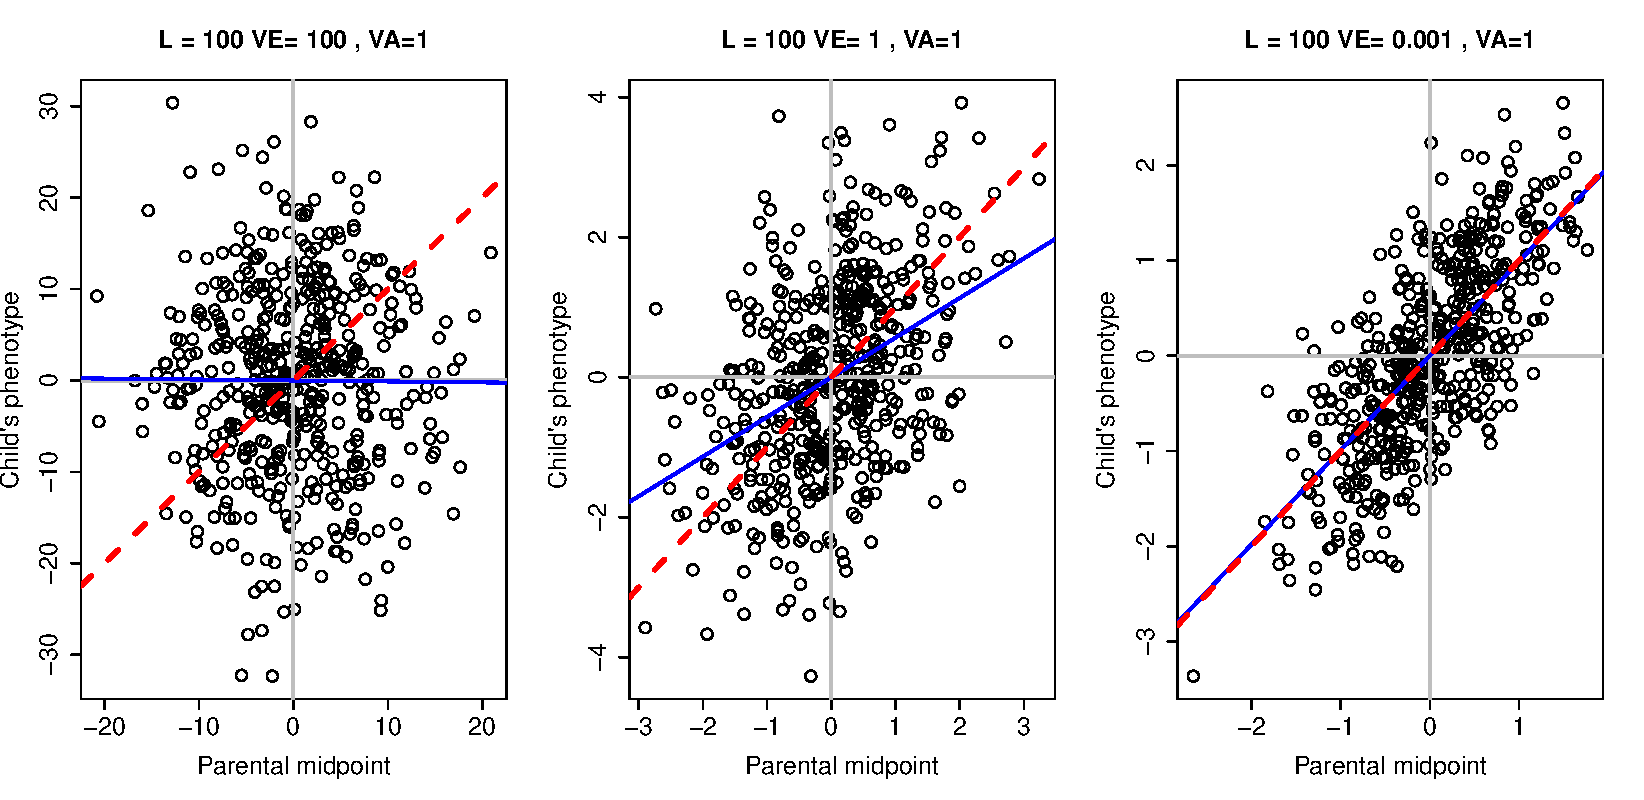
\includegraphics[width=\textwidth]{figures/QT2.pdf}
\end{center}
\caption{Regression of child's phenotype of the parental mid-point phenotype. The three panels show decreasing levels of environmental
  variance ($V_E$) holding the additive genetic variance constant ($V_A=1$). 
 In these figures, we simulate $100$ loci, as described in
 the caption of Figure \ref{fig:QT1}.We simulate the genotypes and
 phenotypes of the two parents, and then simulate the child's genotype
following mendelian transmission. The red line shows $x=y$ and the blue
line shows the best fitting linear regression
line. \gitcode{https://github.com/cooplab/popgen-notes/blob/master/Rcode/Quant_gen/QT2.R}
} \label{fig:midpar}
\end{figure}


Applying this heritability estimate to the Song sparrow sample we find
$h^2=0.43$ and $h^2=0.3$ for beak depth and tarsus length
respectively from Figure
\ref{fig:song_sparrow_herit}. So in \citet{smith1979heritability} analysis, for example,
$30\%$ of the variance in tarsus length is atttributal to the additive
effect of genetic
differences among individuals. 
\citet{smith1979heritability} also regressed the average offspring
phenotype agains their fathers {\emph or} mothers against their
offspring, giving a slope of $\beta_{\textrm{dad}, \textrm{avg. kid}}$ and
$\beta_{\textrm{mum}, \textrm{kid}}$, and for tarsus length, for
example, they found $\beta_{\textrm{dad},
  \textrm{avg. kid}}= 0.19$ and $\beta_{\textrm{mum},
  \textrm{avg. kid}}= 0.17$.  Following a similar argument to
that in eqn
\eqref{eqn:par_off_herit} we find that these slopes are $\beta_{\textrm{dad}, \textrm{kid}}=
\nicefrac{\nicefrac{V_{A}}{2}}{V} = \nicefrac{h^2}{2}$, and the same
  for mums. Thus the regression of offspring's phenotype on a
  particular parent is an estimate of half the narrow-sense
  heritability, in line with the reduced slopes found by
  \citet{smith1979heritability}, this halfing of the slope is due to the
  fact that a single parent's phenotype is a noisier estimate of the
  parental mid-point and so less informative about the child
  s phenotype. These parent specific estimates of heritability are
  particularly useful as they allow us to investigate sex-specific inheritance and sexual
  dimorphism (we'll explore this in a later section). 


 \begin{marginfigure}
\begin{center}
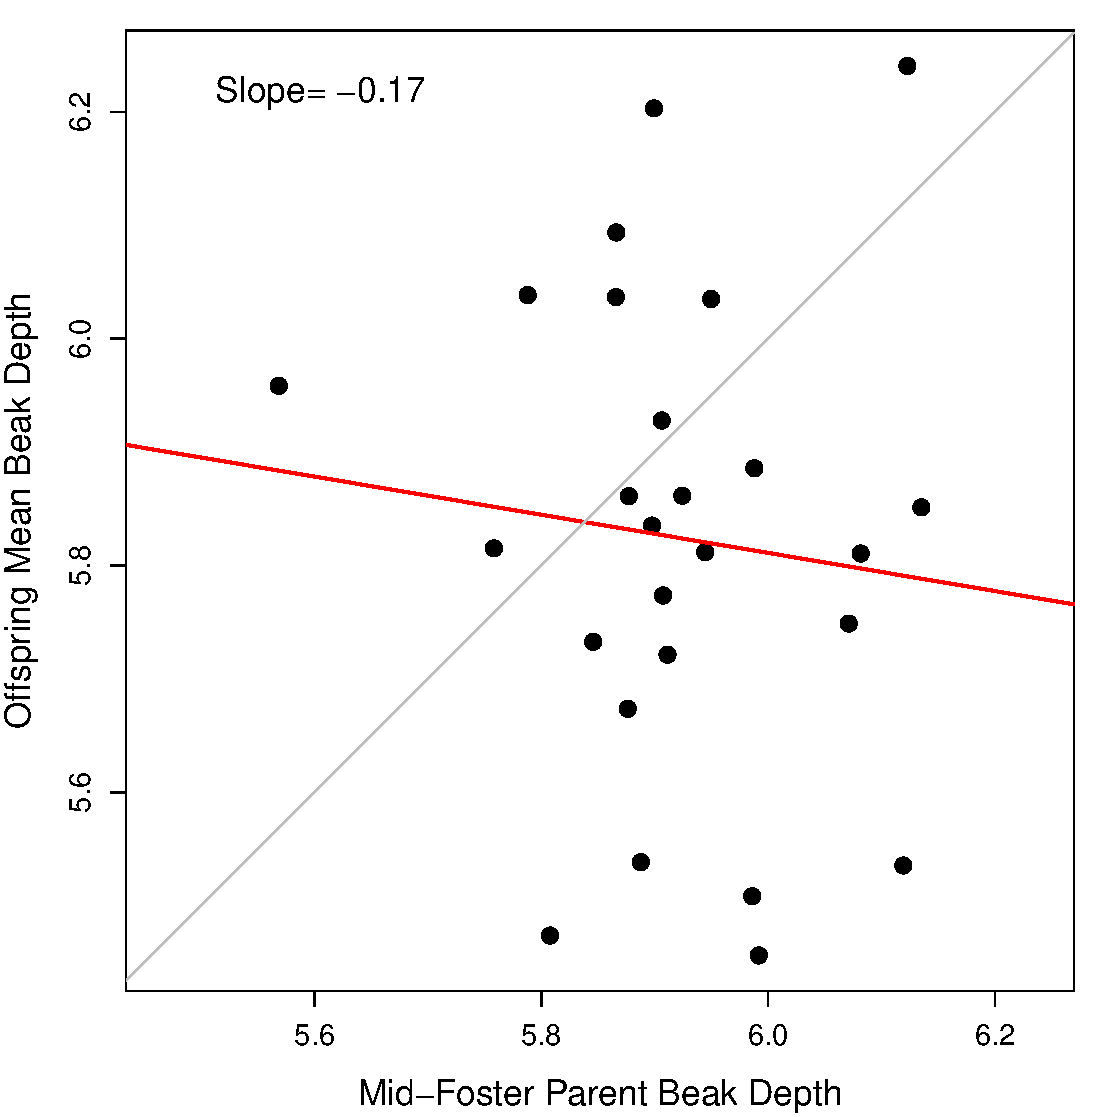
\includegraphics[width=\textwidth]{Journal_figs/Quant_gen/song_sparrow_herit/song_sparrow_herit_foster.pdf}
\end{center}
\caption{Foster Parent-midpoint offspring regression for beak depth and
  tarsus length in song sparrows. The red line shows the best fitting
  slope, whose slope is reported on the graph. The slope is not significant. The grey line is the
  $x=y$ line. Data from \citet{smith1980experimental},
  \gitcode{https://github.com/cooplab/popgen-notes/blob/master/Journal_figs/Quant_gen/song_sparrow_herit/song_sparrow_herit.R}} \label{fig:song_sparrow_herit_foster}
\end{marginfigure}


Estimating heritability by these various parent-offspring regression have the issue of not controlling for
environmental correlations between parent and offspring, which can
inflate our estimates of heritability (as we will mistake
environmentally mediated resemblance for genetics). Raising the
organisms in the lab could remove much of the potential for shared
environment between parent and offspring, but it also removes much of the
environmental variation and we (as evolutionary geneticists) are usually not primarily interested in knowing
the heritability in the lab bur rather in the field. In some organisms,
notably plants, we can begin to sidestep these issues by raising offspring
in a common set of randomized field conditions (a so called ``common
garden''). Another option is cross-foster animals, for example
\citet{smith1980experimental} returned to the song sparrow population
and swapped eggs between parents nests. They found that the covariance
between biological parents and children was still high despite these
children being raised in a different nest, but that there was no significant
covariance between foster parents and their non-biological children
(see Figure \ref{fig:song_sparrow_herit_foster} for beak depth). This suggests that
family environment is not confounder in estimating the heritability in
this song sparrow sample. However, such manipulations are often
impossible in many systems, and issues of shared environmental
covariance due to maternal resources from egg (or seed) are still present. 

Despite its issues, this measure of heritability provides useful
intuition and is directly relevant to our discussion of the response to selection in
the next chapter. That's because our regression allows us to attempt to predict the phenotype of the
child given the phenotypes of the parents; how well we can do this depends on the
slope. See Figure \ref{fig:midpar} for examples. If the slope is close to zero then the parental phenotypes hold no
information about the phenotype of the child, while if the slope is
close to one then the parental mid-point is a good guess at the child's
phenotype. As we will see, natural selection will only efficiently
drive evolution if children resemble their parents.\\

Thinking abour our prediction of child's phenotpye more formally, the expected phenotype of the child given the parental
phenotypes is
\begin{equation}
\E(X_{kid} | X_{mum},X_{dad}) = \mu +
\beta_{mid,kid}(X_{mid} - \mu) =\mu + h^2(X_{mid} - \mu)  \label{predict_kid}
\end{equation}
which follows from the definition of linear regression. So to find the
child's predicted phenotype, we simply take the mean phenotype and add on the difference between our parental mid-point and the population mean, multiplied by our
narrow sense heritability. \\


\begin{question}
Briefly explain what Galton meant by 'regression towards
mediocrity', and why he observed this pattern in light of Mendelian inheritance.
\end{question}



\paragraph{The covariance between general pairs of relatives under an
additive model}


The above examples above make clear that to understand the covariance between
phenotypes of relatives, we simply need to think about the alleles they
share IBD. Consider a pair of relatives ($1$ and $2$) with a probability $r_0$,
$r_1$, and $r_2$ of sharing zero, one, or two alleles IBD
respectively. When they share zero alleles
$Cov((X_{1M}+X_{1P}),(X_{2M}+X_{2P}))=0$, when they share one allele
$Cov((X_{1M}+X_{1P}),(X_{2M}+X_{2P}))=
Var(X_{1M})=\frac{1}{2}V_A$, and when they share two alleles $Cov((X_{1M}+X_{1P}),(X_{2M}+X_{2P}))=
V_A$. Therefore, the general covariance between two
relatives is
\begin{equation}
Cov(X_1,X_2) = r_0 \times 0 + r_1 \frac{1}{2}V_A + r_2  V_A =
2 F_{1,2} V_A  \label{additive_covar_general_rellys}
\end{equation}\\ 
%% Need to define F 1,2 -- EBJ
So under a simple additive model of the genetic basis of a phenotype,
to measure the narrow sense heritability we need to measure the
covariance between pairs of relatives (assuming that we can remove the effect of
shared environmental noise). From the covariance between relatives we
can calculate $V_A$, and we can then divide this by the total phenotypic
variance to get $h^2$. \\
%One way potentially to get somewhat around the
%shared environmental effect is to use paternal half-sibs as they share a

 
\begin{question}
{\bf A)} In polygynous red-winged blackbird populations (i.e. males mate with
several females), paternal half-sibs can be identified.  Suppose that
the covariance of tarsus lengths among half-sibs is 0.25 $cm^2$ and
that the total phenotypic variance is 4 $cm^2$.  Use these data to
estimate $h^2$ for tarsus length in this population. \\

{\bf B)} Why might paternal half-sibs be preferable for measuring
heritability than maternal half-sibs? 
\end{question}
\begin{marginfigure}[-2cm]
\begin{center}
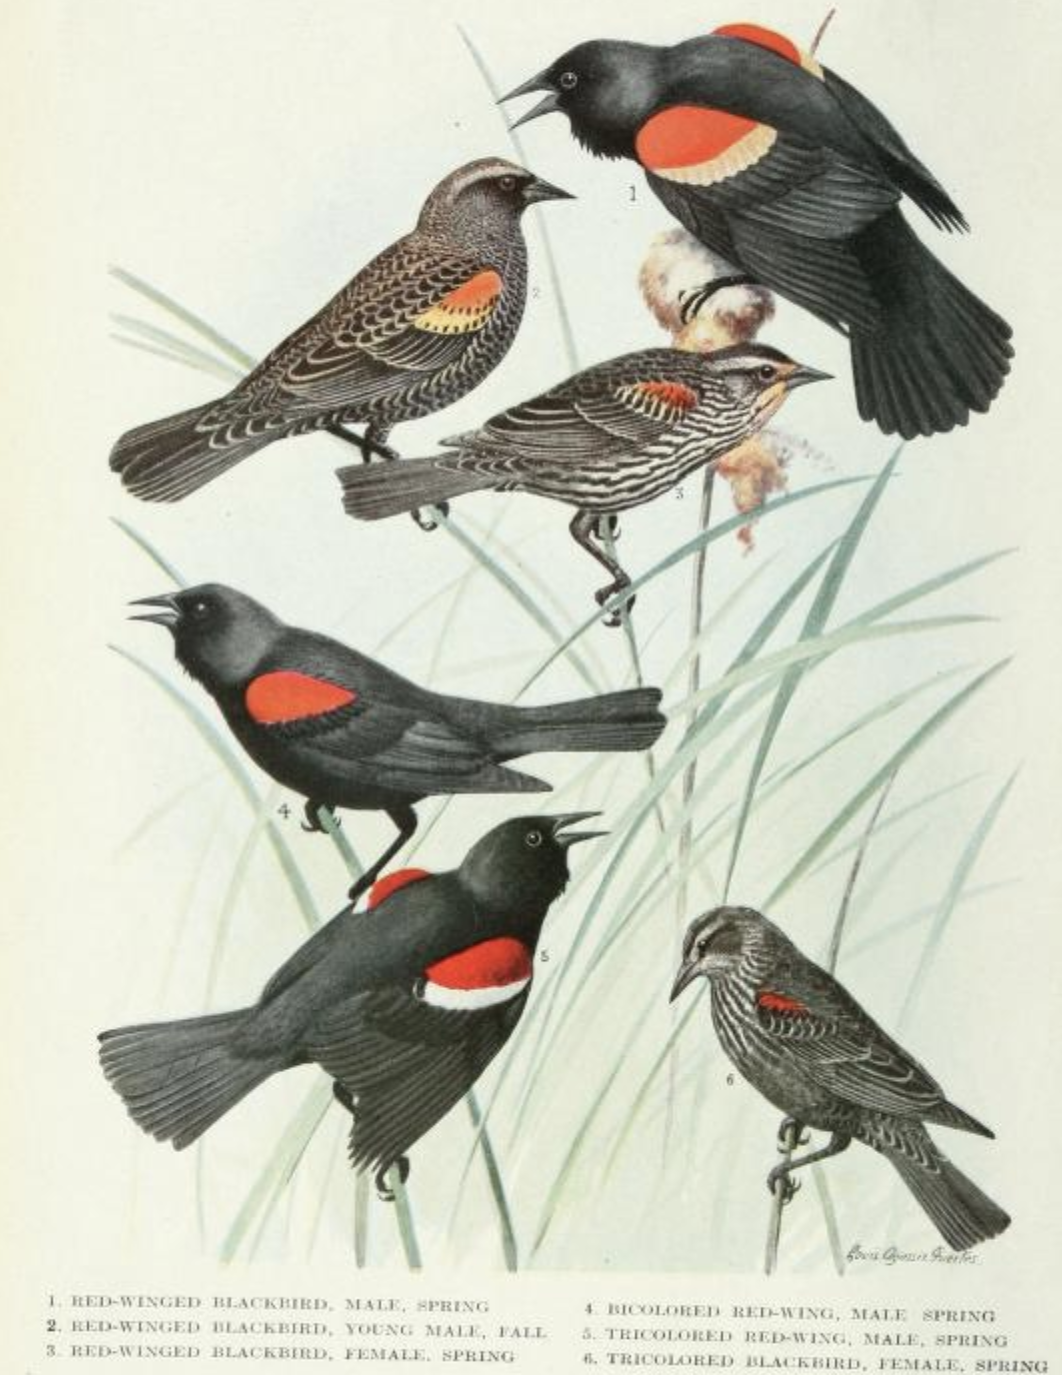
\includegraphics[width=\textwidth]{illustration_images/Quant_gen/red_winged_blackbirds/Red_wing_blackbirds.png}
\end{center}
\caption{Red-winged blackbird and Tricoloured Red-winged blackbirds
  ({\t Agelaius phoeniceus} and {\it Agelaius tricolor}). \BHLNC{Bird-lore (1899). National Association of Audubon Societies for the Protection of Wild Birds and Animals.}{https://archive.org/stream/birdlore24nati/birdlore24nati\#page/n89/mode/1up}{American Museum of Natural History Library}}\label{fig:RW_blackbird}
\end{marginfigure}

\paragraph{Estimating additive genetic variance across a variety of
  different relationships (The animal model).}

In many natural populations we may have access to individuals with a
range of different relationships to each other (e.g. through monitoring
of the paternity of individuals), but relatively few pairs of individuals for a specific relationship (e.g. sibs). We can try and use this information on various relatives as
fully as possible in a mixed model framework. Building from equation
\ref{pheno_geno_environ}, we can write an individual's phenotype $X_i$
 as 
\begin{equation}
X_i =  \mu  + X_{A,i} + X_{E,i} 
\end{equation}
where $X_{E,i} \sim N(0,V_E)$  and $X_{A,i}$ is normally distributed across
individuals with covariance matrix $V_A A$, where the the entries for
a pair of individuals i and j are 
$A_{ij}= 2 F_{i,j}$ and $A_{ii}= 1$. Given the matrix $A$ we can estimate $V_A$. We can
also add fixed effects into this model to account for generation
effects, additional mixed effects could also be included to account
for shared environments between particular individuals (e.g. a shared nest).
This approach is sometimes called the ``animal model'', and is widely
used to in modern quantitative gentics to estimate genetic variances and heritabilities. 


%% plot of covariance of human traits for different relationships https://www.nature.com/articles/s41539-017-0005-6/figures/1

\section{Multiple traits}
Traits often covary with each other, both due to environmentally
induced effects (e.g. due to the effects of diet on multiple traits)
and due to the expression of underlying genetic covariance between
traits. Genetic covariance, in turn, can reflect pleiotropy, a
mechanistic effect of an allele on multiple traits (e.g. variants that
affect skin pigmentation often affect hair color), the genetic
linkage of loci independently affecting multiple traits, or the
effects of assortative mating. 

Consider two traits $X_{1,i}$ and $X_{2,i}$ in an individual $i$. These traits could be,
say, the individual's leg length and nose length. As before, we can write
these as 
\begin{eqnarray}
X_{1,i} &= \mu_1+ X_{1,A,i} + X_{1,E,i}  \nonumber \\
X_{2,i} &= \mu_2 +X_{2,A,i} + X_{2,E,i} \nonumber \\
\end{eqnarray}
As before we can talk about the total phenotypic variance ($V_1,V_2$),
environmental variance  ($V_{1,E}$ and $V_{2,E}$), and the additive genetic variance for trait one and two ($V_{1,A}$, $V_{2,A}$). But now we also have to consider the 
total covariance between trait one and trait two, $V_{1,2}=Cov(X_{1},X_{2})$, as well as the environmentally induced covariance ($V_{E,1,2}=Cov(X_{1,E}
,X_{2,E} )$) and the additive genetic covariance ($V_{A,1,2}
=Cov(X_{1,A} ,X_{2,A} )$). To better understand the covariance arising due to pleiotropy, let's think about a set of $L$ SNPs contributing to our two traits. If the additive effect of an allele at the $i^{th}$ SNP is $\alpha_{i,1}$ and $\alpha_{i,2}$ on traits 1 and 2, then the additive covariance between our traits is
\begin{equation}
V_{A,1,2} = \sum_{i=1}^L 2\alpha_{i,1}\alpha_{i,2} p_i(1-p_i)
\end{equation}
assuming our loci are in linkage disequilibrium. Thus a genetic
correlation arises due to pleiotropy, because loci that tend to affect
trait 1 also systematically affect trait 2. For example, alleles
associated with later Age at Menarche (AAM) in European women also
tend to be positively associated with height (see Figure
\ref{fig:AAM_height}), thereby creating a genetic correlation between
AAM and height. 

\begin{marginfigure}
\begin{center}
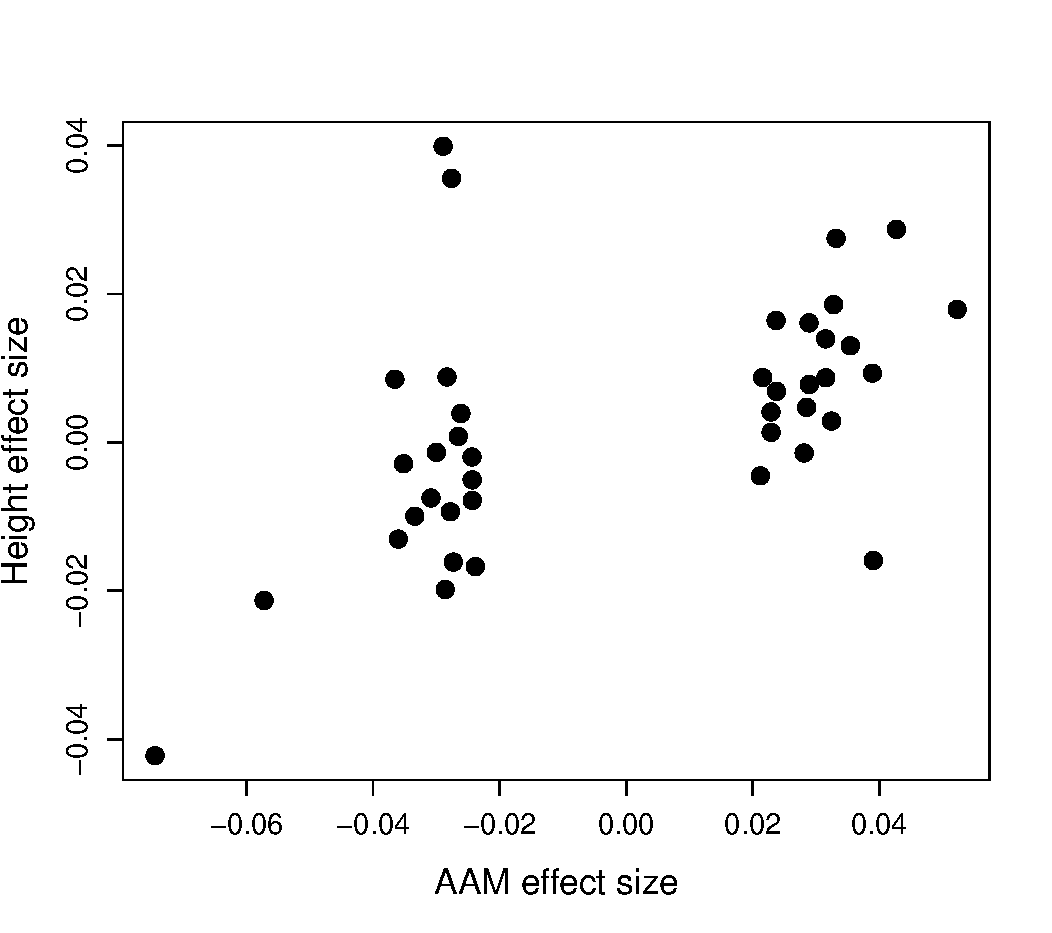
\includegraphics[width= \textwidth]{Journal_figs/Quant_gen/pickrell_pleiotropy/AAM_height.pdf}
\end{center}
\caption{The additive effect sizes of loci associated with female Age
  at Menarche (AAM) and their effect size on Height in a European
  population. Data from \citet{pickrell2016detection}. \gitcode{https://github.com/cooplab/popgen-notes/blob/master/Journal_figs/Quant_gen/pickrell_pleiotropy/AAM_height_pickrell.R}} \label{fig:AAM_height}   
\end{marginfigure}

We can store our variance and covariance values in matrices, a way of gathering these terms that will be useful when we discuss selection: 
\begin{equation}
\bf{V}= \left( \begin{array}{cc} 
V_{1} & V_{1,2} \\
V_{1,2} & V_{2} \\
\end{array} \right) \label{P_matrix}
\end{equation}
and
\begin{equation}
\bf{G}= \left( \begin{array}{cc} 
V_{1,A} & V_{A,1,2} \\
V_{A,1,2} & V_{2,A} \\
\end{array} \right)  \label{G_matrix}
\end{equation}
Here we've shown the matrices for two traits, but we can generalize this to an arbitrary number of traits.

We can estimate these quantities, in a similar way as before, by
studying the covariance in different traits between relatives: 
\begin{equation}
Cov(X_{1,i},X_{2,j}) = 2 F_{i,j} V_{A,1,2}
\end{equation}
\begin{marginfigure}
\begin{center}
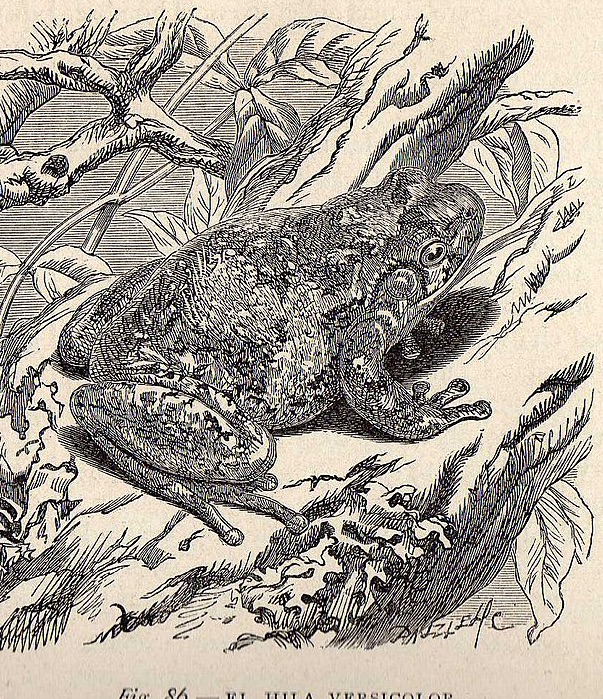
\includegraphics[width= \textwidth]{illustration_images/Quant_gen/Hyla_versicolor/Hyla_versicolor.jpg}
\end{center}
\caption{Grey treefrog
  ({\it Hyla versicolor})
  \wikimedia{Historia Natural, tomo V ``Reptiles y peces'' (1874) Juan Vilanova y Piera,  p. 156. 
  }{https://commons.wikimedia.org/wiki/Category:Hyla_arboricola\#/media/File:Hyla_arboricola_and_Hyla_versicolor.jpg}{Dorieo}{Cropped. Public
  Domain}} \label{fig:Hyla_versicolor}   
\end{marginfigure}  %% right book ref https://books.google.com/books?id=f6lrVNHsNUcC&pg=PP7&lpg=PP7&dq=Juan+Vilanova+y+Piera+y+otros,+Historia+Natural,+tomo+V+%22Reptiles+y+peces%22&source=bl&ots=QzpSB7umN_&sig=ACfU3U3cE95FUKtWlt_PpgE-wCTmwHSMnw&hl=en&sa=X&ved=2ahUKEwiw392pq_LmAhXDqp4KHRrNDLgQ6AEwDXoECAoQBA#v=onepage&q=Juan%20Vilanova%20y%20Piera%20y%20otros%2C%20Historia%20Natural%2C%20tomo%20V%20%22Reptiles%20y%20peces%22&f=false
An example of phenotype and genetic covariance are shown on the left
and right of Figure \ref{fig:Frog_genetic_corr} respectively. Gray
treefrogs ({\it Hyla versicolor}) chorus to attract mates. Their call
is made up of a trill, a note rapidly pulsed a number of times, that
is then repeated after some
period. Female frogs prefer males who make a lot of calls and where each
of those calls have a large number
of pulses. However, doing both is be very energetic, and so
there is potentially a tradeoff between these two aspects of a male frog's
call. Indeed \citet{welch2014multivariate} found
in lab-reared male frogs that the pulse number and the time period between
calls were positively correlated, left side of Figure \ref{fig:Frog_genetic_corr}, i.e. individuals were investing
their energy in making either few highly pulsed calls or many calls
with few pulses. This phenotypic covariance reflects underlying a
genetic covariance between theses two frog call
characteristics (right side  Figure \ref{fig:Frog_genetic_corr}). Fathers whose sons have calls with highly pulsed
calls also have sons whose calls are more spaced apart.

%% Hyla
%https://www.flickr.com/photos/internetarchivebookimages/18193065982/in/photolist-tHEdFq-w6oVxt-w7uzuh-wYEMiJ-wM1ydg-tDzszv-wM68MH-w7zib5-x4zbJZ-x3NmSS-toJn5T-ymBaUK-x2gbjQ-tHGbU5-w7zFrh-wDq3dw-wpp5b5-x3GxoJ-xieMpX-x52jC8-x3JEB7-x2b6Bo-w7tkef-wLSL61-toKL3z-w7Ekq4-tFd8h6-vdPjbF-x4sbkM-wLSNwy-wM1vjR-truv4Z-w7CJTR-w7Bk7p-xjs4Gw-tHH1k7-xCgp7d-wLTGnA-xAeJRf-sJnrKP-tFB9xC-wLuk1W-w7tDKd-x15TQs-wLWVow-toz9Lb-xBEY7g-xhGSS2-x15Vsq-x56QhF
%% https://www.flickr.com/photos/internetarchivebookimages/20225306138/in/photolist-tJ4Rn4-xu7KMN-x4sHmz-x29vVY-xgVebh-wLukBA-xx36Hr-uyhbMs-wLYycD-x1cYNP-wkFrYW-wLSya7-wEMZoc-wLsZrX-x16hfW-x3cPhW-xDWcZt-xmB6i6-wvustq-xqaxeV-xoyLPh-x79DmT-x79CR4-wrM4wH-x72MZu-wYAHWG-xfDTP6-xfDTkv-xfDSSX-wXogss-xeYxDi-x8acmV-wb8XiL-wQEAzM-x5QBpL-wb8Gsd-wQwQbj-x71pJS-wQacmE-x6X6Si-wPeYSN-x4w3xq-wJ7vQC-w4EZxA-otAReB-oeFYJM-ovuHRw-otT3ar-otAQJZ-otAQmV
% https://upload.wikimedia.org/wikipedia/commons/c/c8/Hyla_arboricola_and_Hyla_versicolor.jpg
\begin{figure}
\begin{center}
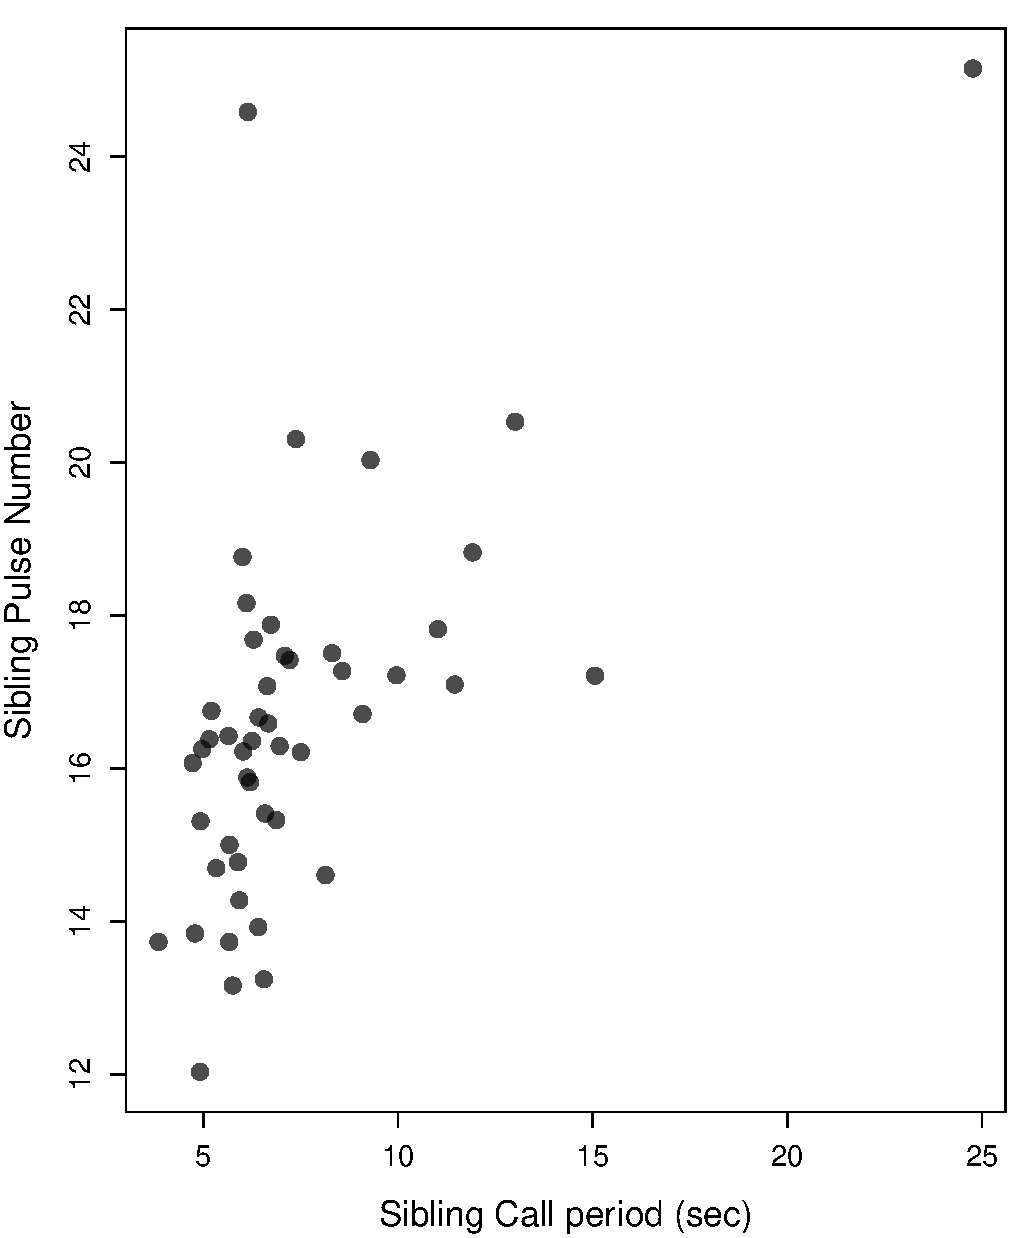
\includegraphics[width= \textwidth]{Journal_figs/Quant_gen/Frog_calls_Hyla_versicolor/Frog_calls_sibling_means.pdf}
\end{center}
\caption{Phenotypic and Genetic correlations in male grey treeforg
  ({\it Hyla versicolor}) calls. On the left each male is shown as a
  dot, recording their inter-call period and the number of pulses in each call. One
  the right each dot corresponds to a father with the mean of sons
  for both phenotypes. Data from \citet{welch2014multivariate} downloaded from
\href{https://datadryad.org/stash/dataset/doi:10.5061/dryad.40sj6}{dryad}, \gitcode{https://github.com/cooplab/popgen-notes/blob/master/Journal_figs/Quant_gen/Frog_calls_Hyla_versicolor/Frog_calls_Hyla_versicolor.R}} \label{fig:Frog_genetic_corr}  
\end{figure}
% https://commons.wikimedia.org/wiki/File:Hyla_arboricola_and_Hyla_versicolor.jpg


One useful summary of a genetic covariance is the genetic correlation between two phenotypes
\begin{equation}
r_g = \frac{V_{A,1,2}}{\sqrt{V_{A,1}V_{A,2}}}
\end{equation}
where $V_{A,1}$ and $V_{A,2}$ are the additive genetic variance for trait 1 and 2 respectively. Here, $r_g$ tells us to what extent the additive genetic variance in two traits is correlated.   



Another important application of genetic covariances is in the
study of sexually antagonistic selection and the evolution of sexual
dimorphism, here we'll calculate the genetic covariance between male and female phenotypes. For example, below is the relationship between the forehead patch size for Pied fly-catcher fathers and their sons and daughters. The phenotype has been standardized to have mean $0$  and variance $1$ in each group. The phenotypic covariance of the sample of fathers and sons is $0.35$, while the phenotypic covariance of fathers and daughter is $0.23$. 



\begin{figure}
\begin{center}
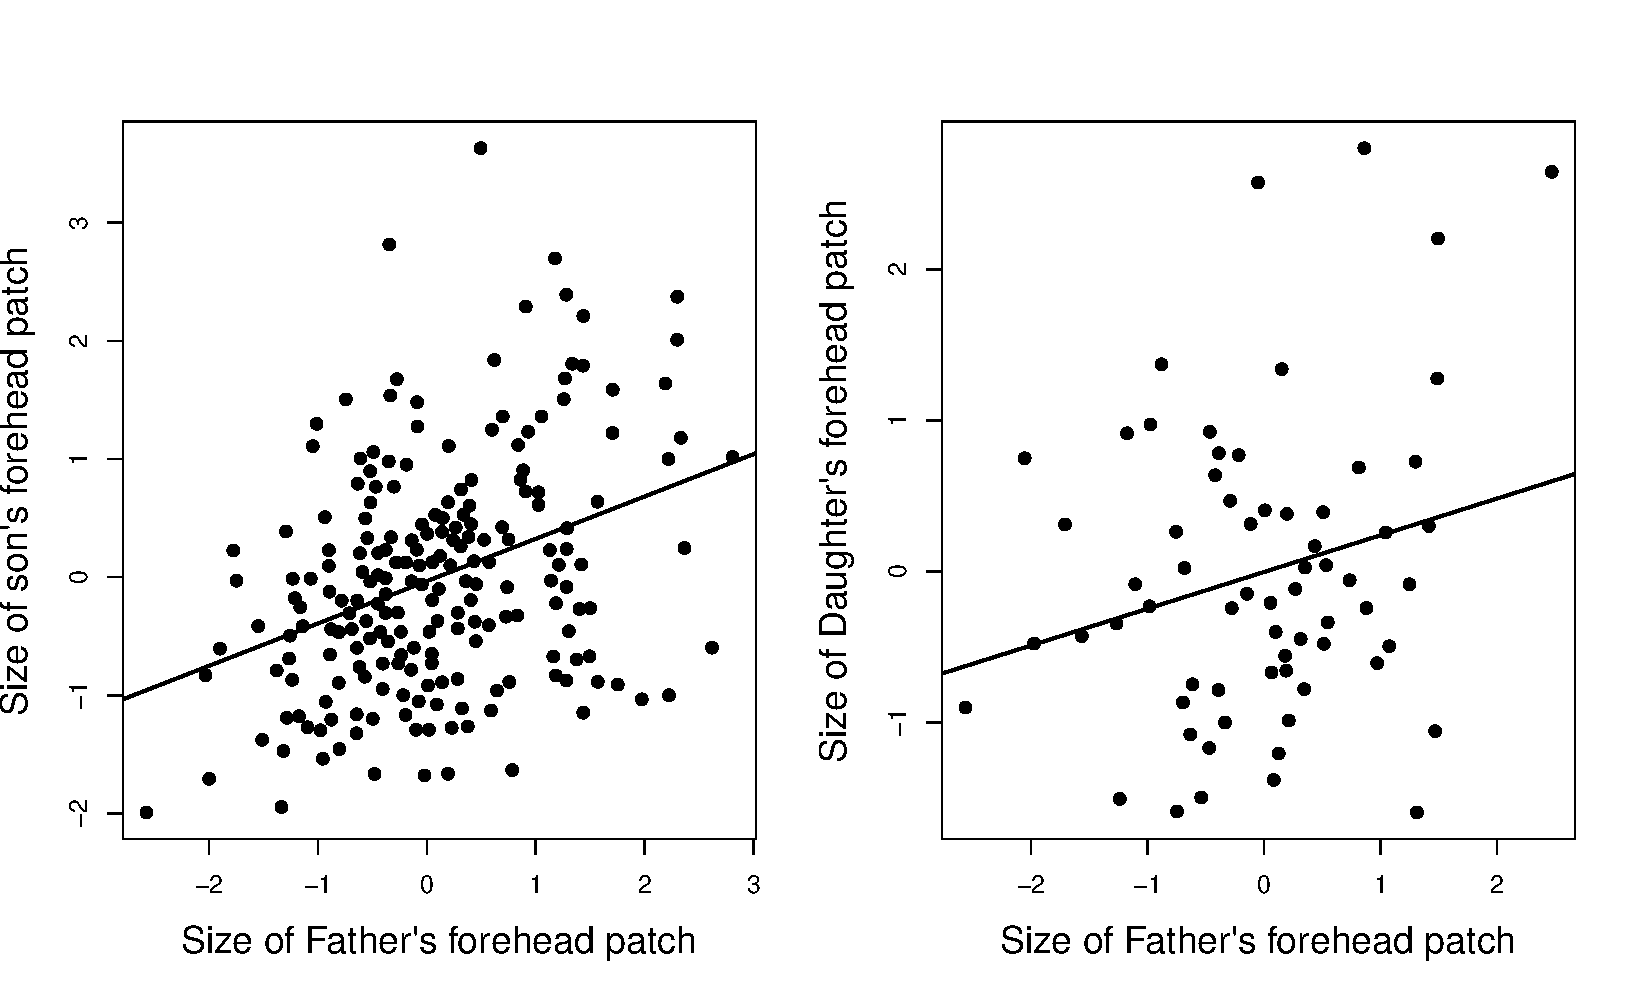
\includegraphics[width= \textwidth]{Journal_figs/Quant_gen/pied_fly_catcher_sex_genetic_corr/FlyCatcher_genetic_corr.pdf}
\end{center}
\caption{Relationship of standardized forehead patch size between
  fathers and sons and daughters in  Pied fly-catchers. Data from
  \citeauthor{potti:11}. \gitcode{https://github.com/cooplab/popgen-notes/blob/master/Journal_figs/Quant_gen/pied_fly_catcher_sex_genetic_corr/Potti_Canal_2011_sex_cov.R}} \label{fig:FlyCatcher_genetic_corr}   %\cite{potti:11} 
\end{figure}

\begin{marginfigure}
\begin{center}
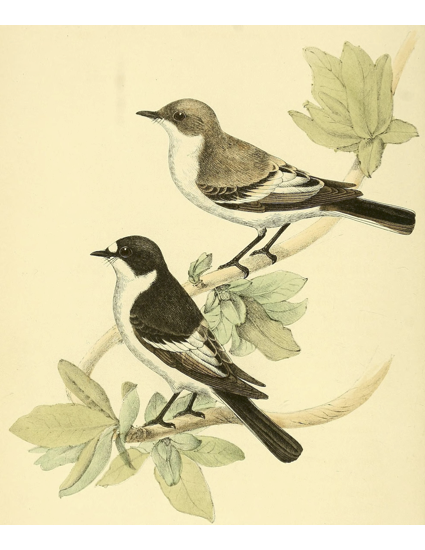
\includegraphics[width=0.9
\textwidth]{illustration_images/Quant_gen/pied_fly_catcher/pied_fly_catcher.png}
\end{center}
\caption{{\it Ficedula hypoleuca}, Pied fly-catcher.  \BHLNC{Coloured
    illustrations of British birds, and their eggs (1842-1850).
London :G.W. Nickisson. }{https://www.biodiversitylibrary.org/page/40246319\#page/335/mode/1up}{Smithsonian Libraries}} \label{fig:FlyCatcher}   %% not
                                %% sure if it's a female or juv. https://www.biodiversitylibrary.org/page/40246319#page/334/mode/1up
\end{marginfigure}

\begin{question}
Assume we can ignore the effect of the shared environment in our Pied fly-catcher example. \\
{\bf A)} What is the additive genetic covariance between male and female patch size?\\
{\bf B)} What is the additive genetic correlation of male and female patch size? You can assume that the additive genetic variance is the same in males and females.
\end{question}
\subsection{Non-additive variation.}
\label{section:nonAddVar}
Up to now we've assumed that our alleles contribute to our phenotype in an
additive fashion. However, that does not have to be the case as there may be
non-additivity among the alleles present at a locus (\emph{dominance}) or among
alleles at different loci (\emph{epistasis}). We can accommodate these complications
into our models. We do this by partitioning our total genetic variance into
independent variance components.


%, such that the phenotype of the genotype of the heterozyote is the
%same as the $11$ homozygote. The area of each circle is proportion to the
%fraction of the population in each genotypic class ($p^2$, $2pq$, and $q^2$). 

\paragraph{Dominance.} To understand the effect of dominance, let's consider how the allele
that a parent transmits influences their offspring's
phenotype. A parent transmits one of their two alleles at a locus to their offspring. 
Assuming that individuals mate at random, this allele is paired with another allele drawn at random from the population.
For example, assume your mother transmitted an allele 1 to you: with probability $p$ it would be paired with another allele 1, and you would be a homozygote; and with probability $q$ it's paired with a 2 allele and you're a heterozygote.

%The first variance component is the variance due to
%the additive contribution of each allele ($V_A$). 

Now consider an autosomal biallelic locus $\ell$, with frequency $p$ for allele 1, and
genotypes $0$, $1$, and $2$ corresponding to how many copies of allele
$1$ individuals carry. We'll denote the mean phenotype of an individual
with genotype $0$, $1$, and $2$ as $\overline{X}_{\ell,0}$,
$\overline{X}_{\ell,1}$, $\overline{X}_{\ell,2}$ respectively. This mean is
taking an average phenotype over all the environments and genetic backgrounds the alleles
are present on. We'll mean center (MC)
these phenotypic values, setting $\overline{X}'_{\ell,0} = \overline{X}_{\ell,0} - \mu$, and
likewise for the other genotypes. 

We can think about the average
(marginal) MC
phenotype of an individual who received an allele 1 from their parent as the average of the MC phenotype for heterozgotes and 11 homozygotes, weighted by the probability that
the individual has these genotypes, i.e. the probability they receive an additional allele $1$ or an allele $2$ from their other parent:
\begin{equation} 
  a_{\ell, 1} = p\overline{X}'_{\ell,2}  + q\overline{X}'_{\ell,1},
\end{equation}
Similarly, if your parent transmitted an 2 allele to you, your average
MC phenotype would be
\begin{equation}
  ~~ a_{\ell, 2} = p\overline{X}'_{\ell,1}  + q\overline{X}'_{\ell,0} 
\end{equation}

%the marginal value for allele 1, $a_{\ell, 1}$,  follows from the fact that (assuming HW) an allele 1 will be
%paired with another allele 1 with probability $p$, resulting in a
%genotype $11$ (with phenotypic deviation $\overline{X}'_{\ell,2}$) and will
%be paired with an allele 2 with probability $q$ in a heterozygote
%(with phenotypic deviation $\overline{X}'_{\ell,1}$). A similar argument
%can be made for $a_{\ell, 2}$. \\

%The additive MC genetic values (breeding values) of genotype 0, 1, and
%2 are then

Let's now consider the average phenotype of an offspring by how many
copies of the allele $1$ they carry
\begin{center}
\begin{tabular}{cccc}
genotype: & 0, & 1, & 2.\\
additive genetic value: & $a_{\ell,2}+ a_{\ell,2}$, & $a_{\ell,1}+a_{\ell,2}$, & $a_{\ell,1}+a_{\ell,1}$   \label{add_values}
\end{tabular}
\end{center}
%
i.e. the mean phenotype of each genotypes' offspring
averaged over all possible matings to other individuals in the
population (assuming individuals mate at random). Theses are the
additive MC genetic values (breeding values) of our genotypes. 
Here we are simply adding up the additive contributions of the alleles present
in each genotype and ignoring any non-additive effects of genotype.

\begin{figure}
\begin{center}
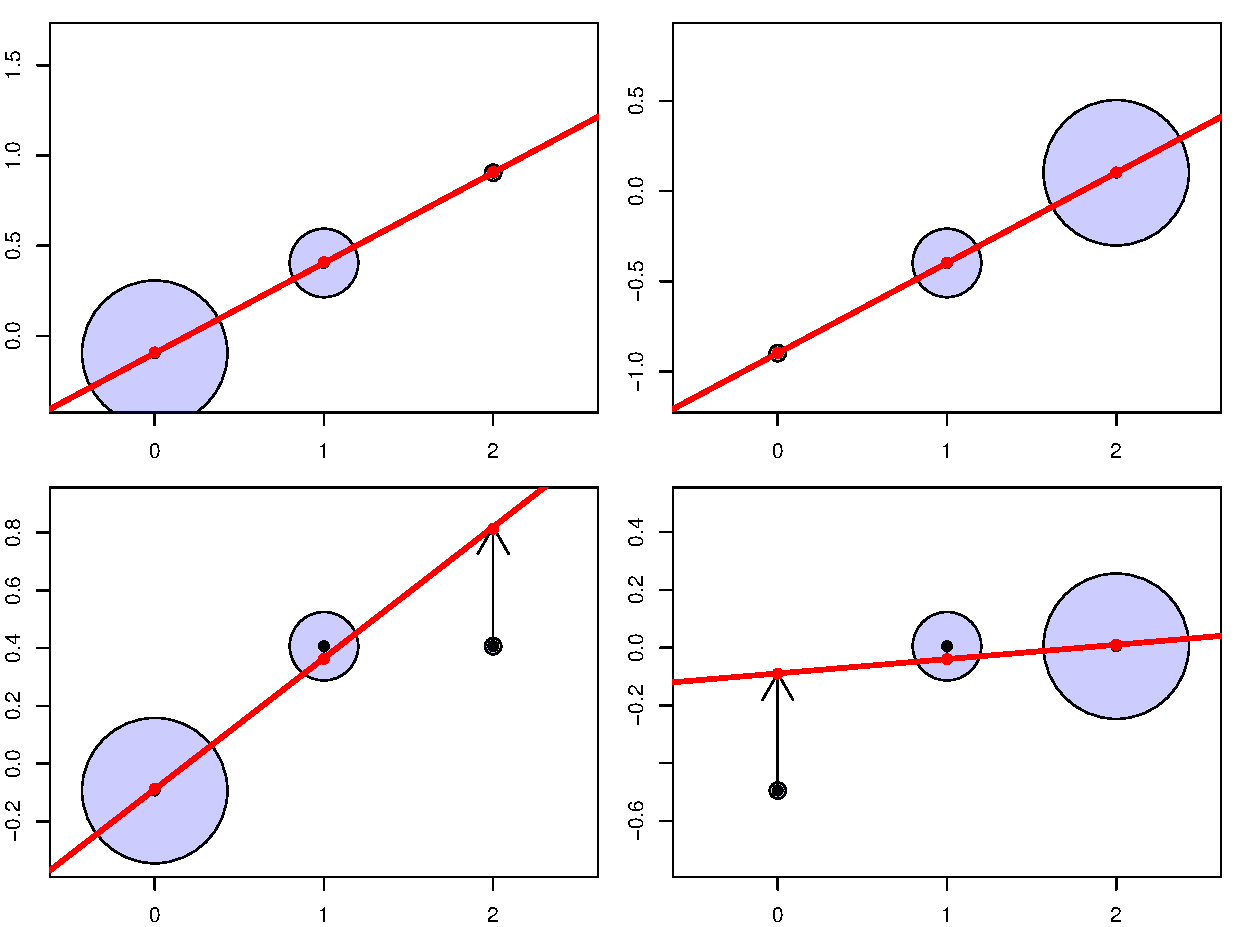
\includegraphics[width=\textwidth]{figures/additive_effect.pdf}
\end{center}
\caption{The average mean-centered (MC) phenotypes plotted against the
  number of allele $1$ carried (from $0$ for $22$ to $2$ for $11$). 
{\bf Top Row:} Additive relationship between genotype and phenotype. 
{\bf Bottom Row:} Allele 1 is dominant over allele 2, such that the
heterozygote has the same phenotype as the $11$ genotype. 
The area of each circle is proportion to the fraction of
the population in each genotypic class ($p^2$, $2pq$, and $q^2$). 
One the left column $p=0.1$ and the right column is $p=0.9$.
The additive genetic values of the genotypes are shown as
  red dots. The regression between phenotype and additive genotype is
  shown as a red line. The black vertical arrows show the difference
between the average MC phenotype and additive genetic value for each genotype. \gitcode{https://github.com/cooplab/popgen-notes/blob/master/Rcode/Quant_gen/additive_effect.R}} \label{fig:add_dom}
\end{figure}


To illustrate this, in Figure \ref{fig:add_dom} we plot two different cases of dominance
relationships; in the top row an additive polymorphism and in the second
row a fully dominant allele. The additive genetic values of the genotypes are shown as red dots. Note that the additive values of the genotypes line up with
the observed MC phenotypic means in the top row, when our alleles interact in a
completely additive manner. Our additive genetic values always fall along a
linear line (the red line in our figure). The additive values are falling along the best
fitting line of linear regression for our population, when phenotype is
regressed against the additive genotype ($0$, $1$, $2$ copies of allele 1)
across all individuals in our population. Note in the dominant case the
additive genetic values differ from the observed phenotypic means, and are
closer to the observed values for the genotypes that are most common in the
population. \\

The difference in the additive effect of the two alleles $a_{\ell, 2}-a_{\ell,
1}$ can be interpreted as an average effect of swapping an allele 1 for an
allele 2; we'll call this difference $\alpha_{\ell}=a_{\ell, 2}-a_{\ell, 1}$.
Our $\alpha_{\ell}$ is also the slope of the regression of phenotype against
genotype (the red line in Figure \ref{fig:add_dom}). Note that the slope of
our regression of phenotype on genotype ($\alpha_{\ell}$)  does not depend on the population
allele frequency for our completely additive locus (top row of
\ref{fig:add_dom}). In contrast, when there is dominance, the slope between
genotype and phenotype ($\alpha_{\ell}$) is a function of allele frequency
(bottom row of \ref{fig:add_dom}). When a dominant allele (1) is rare there is
a strong slope of phenotype on genotype, bottom left Figure \ref{fig:add_dom}.
This strong slope is because replacing a single copy of the 2 allele with a 1
allele in an individual has a big effect on average phenotype, as it will most
likely move an individual from being a 22 homozygote to being a 12
heterozygote. In contrast, when the dominant allele (1) is common in the
population, replacing a 2 allele by a 1 allele in an individual on average has
little phenotypic effect, leading to a weak slope bottom right Figure \ref{fig:add_dom}. This small effect is because as we are mainly turning
heterozygotes into homozygotes (11), who have the same mean phenotype as each other.  \\


\begin{marginfigure}
\begin{center}
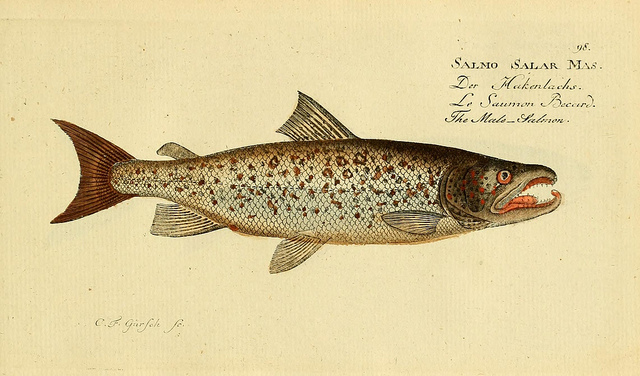
\includegraphics[width=\textwidth]{illustration_images/Quant_gen/Salmon/6918368208_5353868a88_z.jpg}
\end{center}
\caption{Atlantic Salmon ({\it Salmo salar}). \BHLNC{Histoire naturelle des
    poissons. 1796. Bloch,
    M. E.}{https://www.biodiversitylibrary.org/page/4786765\#page/197/mode/1up}{Ernst
    Mayr Library , Museum of Comparative Zoology}} \label{fig:Salmon}
\end{marginfigure}


As as an example of how dominance and population allele frequencies
can change the additive effect of an allele, let's consider the
genetics of the age of sexual maturity in Atlantic Salmon. A single
allele of large effect segregates in Atlantic Salmon that influences
the sexual maturation rate in salmon
\citep{ayllon2015vgll3,barson2015sex}, and hence the timing of their
return from the sea to spawn (sea age). The allele falls close to the
autosomal gene VGLL3 \citep[variation at this gene in humans also
influences the timing of puberty]{cousminer2013genome}. The left side
of Figure \ref{fig:salmon_add_dom} shows the age at  sexual maturity
in males. The L allele associated with slower sexual maturity is recessive in males. While the LL homozygotes mature on average a whole year later, the additive effect of the allele is weak while the L allele is rare in the population. The right panel shows the effect of the L allele in females. Note how the allele is much more dominant in females, and has a much more pronounced additive effect. The dominance of an allele is not a fixed property of the allele but rather a statement of the relationship of genotype to phenotype, such that the dominance relationship between alleles may vary across phenotypes and contexts (e.g. sexes). %\erin{there are no black vertical arrows as referred to in the caption for the salmon dominance figure} 



\begin{figure}
\begin{center}
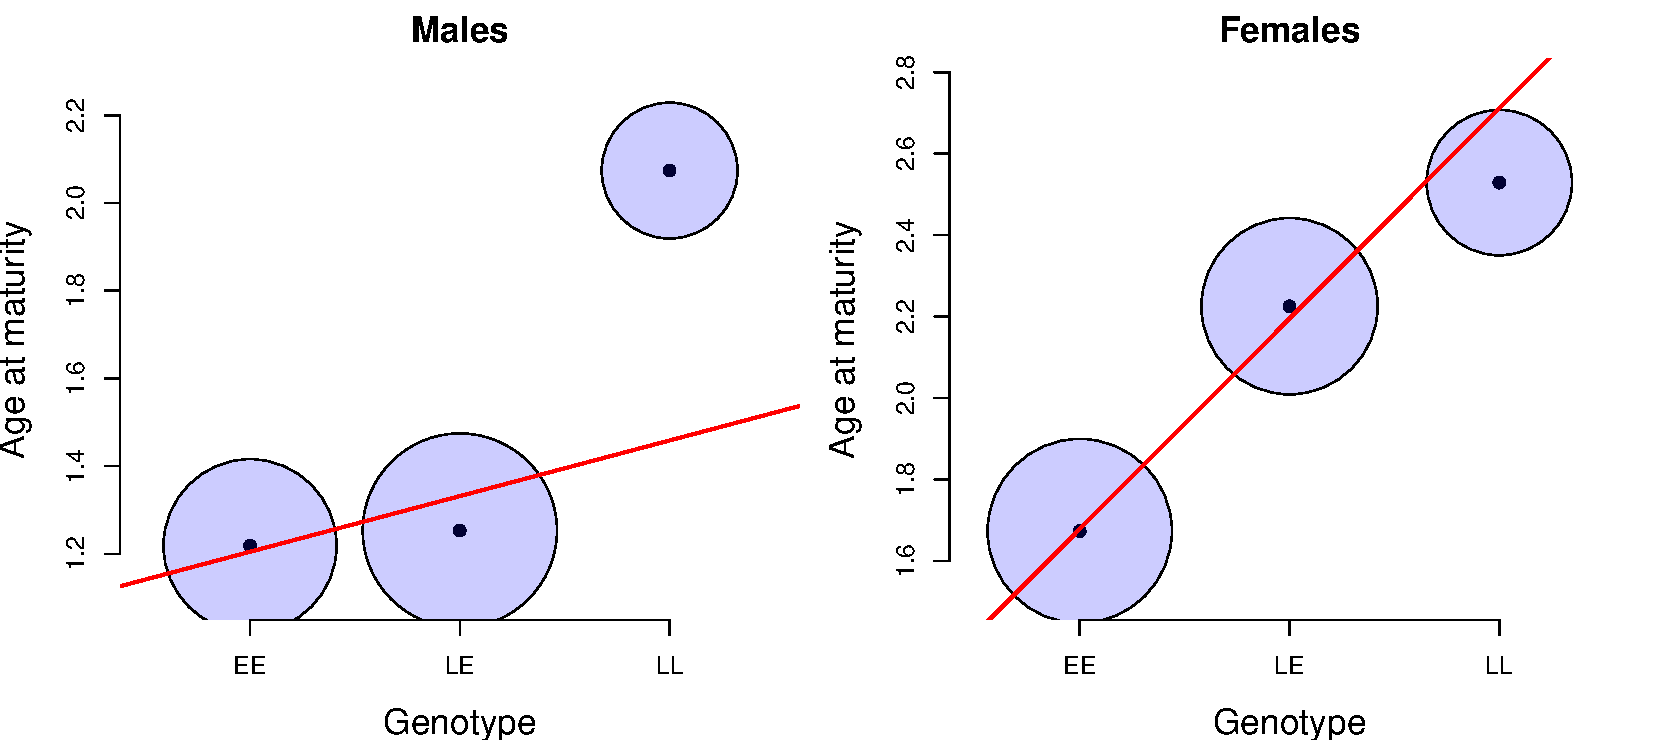
\includegraphics[width=\textwidth]{Journal_figs/Quant_gen/salmon_age/Salmon_age_dom.pdf}
\end{center}
\caption{The average age at sexual maturity for each genotype, broken
  down by sex. 
The area of each circle is proportional to the fraction of
the population in each genotypic class. The regression between phenotype and additive genotype is
  shown as a red line. Data from \citet{barson2015sex}. \gitcode{https://github.com/cooplab/popgen-notes/blob/master/Journal_figs/Quant_gen/salmon_age/Salmon_age.R}} \label{fig:salmon_add_dom} %The black vertical arrows show the difference
%between the average MC phenotype and additive genetic value for each genotype. 
\end{figure}

The variance in the population phenotype due to these
additive breeding values at locus $\ell$, assuming HW proportions, is
\begin{align}
V_{A, \ell} &= p^2 (2a_{\ell,2})^2 + 2pq (a_{\ell,1}+a_{\ell,1})^2 + q^2
(2a_{\ell,0})^2 \nonumber \\
& = 2(p a_{\ell, 1}^2 + q a_{\ell, 2}^2 ) \nonumber \\
& = 2pq \alpha_{\ell}^2
\end{align}
The total additive variance for the whole genotype can
be found by summing the individual additive genetic variances over loci
\begin{equation}
V_A = \sum_{\ell=1}^{L} V_{A, \ell} = \sum_{\ell=1}^{L}
2p_{\ell}q_{\ell} \alpha_{\ell}^2.
\end{equation}

Having assigned the additive genetic variance to be the variance
explained by the additive contribution of the alleles at a locus, we
define the dominance variance as the population variance among
genotypes at a locus due to their deviation from additivity.
We can calculate how much each genotypic mean deviates away from its
additive prediction at locus $\ell$ (the length of the arrows in
Figure \ref{fig:add_dom}). For example, the heterozygote deviates 
\begin{equation}
d_{\ell,1} =\overline{X}'_{\ell,1}  - (a_{\ell,1}+ a_{\ell,2})
\end{equation}
away from its additive genetic value, with similar expressions for
each of the homozygotes ($d_{\ell,0}$ and $d_{\ell,2}$). We can then write the dominance variance at
our locus as the genotype-frequency weighted sum of our squared
dominance deviations
\begin{equation}
V_{D,\ell} = p^2 d_{\ell,0}^2+ 2pq d_{\ell,1}^2+ q^2 d_{\ell,2}^2.
\end{equation}
Writing our total dominance variance as the sum across loci 
\begin{equation}
V_D = \sum_{\ell=1}^{L}  V_{D,\ell}. 
\end{equation}
Having now partitioned all of the genetic variance into additive and
dominant terms, we can write our total genetic variance as 
\begin{equation}
V_{G} = V_A+V_D.
\end{equation}
We can do this because by construction the covariance between our
additive and dominant deviations for the genotypes is zero. We can
define the narrow sense heritability as before
$h^2=V_A/V_P=V_A/(V_G+V_E)$, which is the proportion of phenotypic
variance due to additive genetic variance. We can also define the 
total proportion of the phenotypic variance due to genetic differences
among individuals, as the broad-sense heritability $H^2 =
V_G/(V_G+V_E)$. \\

\begin{table}
\begin{center}
\begin{tabular}{| l | c|}
\hline
Relationship (i,j)$^{*}$ &  $Cov(X_i,X_j)$  \\
\hline
parent--child & $\nicefrac{1}{2} V_A$\\
full siblings &$\nicefrac{1}{2} V_A +\nicefrac{1}{4} V_D$\\
identical (monzygotic) twins & $V_A+V_D$ \\
$1^{st}$ cousins & $\nicefrac{1}{8} V_A$\\
\hline
\end{tabular}
\end{center}
\caption{Phenotypic covariance between some pairs of relatives,
  include the dominance variation. $^{*}$Assuming this is the only relationship
the pair of individuals share (above that expected from randomly
sampling individuals from the population). } % doesn't this implicitly assume an infinite population?
\label{table:domcovar}
\end{table}

When dominance is present in the loci influencing our trait ($V_D>0$), we need to modify our
phenotype covariance among relatives to account for this
non-additivity. Specifically, our equation for the covariance among a
general pair of relatives
(eqn. \ref{additive_covar_general_rellys} for additive variation) becomes
\begin{equation}
 Cov(X_1,X_2) = 2 F_{1,2} V_A + r_2 V_D
\end{equation}
where $r_2$ is the probability that the pair of individuals share 2
alleles identical by descent, making the same assumptions (other than additivity) that we made in deriving
eqn. \ref{additive_covar_general_rellys}.  In table
\ref{table:domcovar} we show the phenotypic covariance for some common
pairs of relatives. The regression of offspring phenotype on parental
midpoint still has a slope $V_A/V_P$. 

Full sibs and parent-offspring have the same
covariance if there is no dominance variance (as they have the same
kinship coefficient $F_{1,2}$). However, when dominance
is present ($V_D>0$), full-sibs resemble each other more than
parent-offspring pairs. That's because parents and offspring share
precisely one allele, while full-sibs can share both alleles (i.e. the
full genotype at a locus) identical by descent. We can attempt to
estimate $V_D$ by comparing different sets of relationships. For
example, non-identical twins (full sibs born at same time) 
should have $1/2$ the phenotypic covariance of identical twins if
$V_D=0$. Therefore, we can attempt to estimate $V_D$ by looking at
whether identical twins have more than twice the phenotypic covariance
than non-identical twins. \\

The most important aspect of this discussion for thinking about
evolutionary genetics is that the parent-offspring covariance is still
only a function of $V_A$. This is because our parent (e.g. the mother) transmits only a
single allele, at each locus, to its offspring. The other allele the
offspring receives is random (assuming random mating), as it comes
from the other unrelated parent (the father). Therefore, the average
effect on the child's phenotype of
an allele the child receives from their mother is averaged over
all possible random alleles the child could receive from their father (weighted by their frequency in the population). Thus we only
care about the additive effect of the allele, as parents transmit only
alleles (not genotypes) to their offspring. This means that the short-term response
to selection, as described by the breeder's equation, depends only on
$V_A$ and the additive effect of alleles. Therefore, if we can
estimate the narrow-sense heritability we can predict the short-term response.
However, if alleles display dominance, our value of $V_A$ will change as alleles at our loci change in frequency, e.g. as dominant alleles become common
in the population their contribution to $V_A$ decreases. Therefore,
if there is dominance our value of $V_A$ will not be constant across generations.

Up to this point we have only considered dominance and not epistasis. However, we can include epistasis in a similar manner (for example among pairs of loci). This gets a little
tricky to think about, so we will only briefly explain it. 
 We can first estimate the additive effect of the
alleles by considering the effect of the alleles averaging over their possible genetic backgrounds (including the other interacting alleles they are possibly paired with), just as before. We can then
calculate the additive genetic variance from this. We can estimate
the dominance variance, by calculating the residual variance among
genotypes at a locus unexplained by the additive effect of the
loci. We can then estimate the epistatic variance by estimating the
residual variance left unexplained among the two locus genotypes after accounting for the additive and dominant deviations calculated from each locus separately. In practice these
high variance components are hard to estimate, and usually small as
much of our variance is assigned to the additive effect. Again we
would find that we mostly care about $V_A$ for predicting short-term
evolution, but that the contribution of loci to the additive genetic
variance will depend on the epistatic relationships among loci.



\begin{question}
How could you use 1/2 sibs vs. full-sibs to estimate $V_D$? Why might
this be difficult in practice? Why are identical vs. non-identical
twins better suited for this? 
\end{question}
\erin{I think this would be a better problem if we gave them numbers for covariances and asked them to estimate V dominance in the first part of this problem. }
\begin{question}
Can you construct a case where $V_A=0$ and $V_D>0$? You need
just describe it qualitatively; you don't need to work out the
math. (tricker question). %\erin{what do you want from this? population fixed for dominant allele is what I thought of}
\end{question}


\newpage
